% Generating a PDF file from this template:
%
% Run the LaTeX pdf tool, e.g., pdflatex StudentReport
% Run the bibliographic tool, e.g., bibtex StudentReport
% Run the glossary tool, e.g., makeglossaries StudentReport
%
% You may need to run these commands several times to resolve 
% compilation dependencies.

\documentclass[a4paper,11pt,twoside]{article}

% Inline the SWT LaTeX style here
\newcommand\includedirectory{resources}
% Author: Eugene Yip
% Last modified: 15 October 2019


% ----------------------------------------------------
% Settings common to all documents
\makeatletter
    \if@twoside%
        \usepackage[a4paper, margin = 2.3cm]{geometry}
    \else%
        \usepackage[a4paper, top = 2cm, bottom = 2.5cm, left = 3cm, right = 3cm, includehead, includefoot]{geometry}
    \fi%
\makeatother

\pdfminorversion=6

% Boolean variables to control the document style
\newif\ifsolutionmode	% To switch between blank answer mode or solution mode
\newif\ifshowmarkingbox	% To switch the marking box beside the allocated marks on or off

\usepackage{graphicx}

\newcommand\swtheader{
	\noindent\raisebox{-1.8ex}{
\includegraphics[height=1cm]{\includedirectory/SWT-Logo}}
	\hfill\parbox{0.7\linewidth}{\centering \heading Lehrstuhl Softwaretechnik \& Programmiersprachen\\Fakult{\"a}t Wirtschaftsinformatik \& Angewandte Informatik}
	\hfill\raisebox{-4ex}{
\includegraphics[height=1.8cm]{\includedirectory/UB-Logo}}
}

\newcommand\swtfullheader[1]{
	\swtheader
	\begin{center}
		{\large \heading #1\\[1ex]\courseacronym: \coursename}\\[3ex]
		{\heading \semesterlong}
	\end{center}
	\rule{\textwidth}{1pt}
	\vspace{0em}
}

\newcommand\swtcompactheader{
	\swtheader
	\begin{center}
		{\large \heading \courseacronym: \coursename}\\[3ex]
	\end{center}
	{\sffamily \lecturer \hfill \semesterlong}
	\newline
	\rule{\textwidth}{1pt}
	\vspace{0em}
}

\newcommand\genericheader[1]{
	\thispagestyle{footeronly}
	\clearpage
	\mbox{}\vspace{-1.5cm}

	\swtcompactheader

	\makemaintitle{#1}
}

% Global definition of headings
\usepackage{fancyhdr}
\setlength{\headheight}{14.5pt}
\pagestyle{fancy}
\lhead{\courseacronym (\semester)} \chead{} \rhead{\documentheader}
\lfoot{\issuedate}                 \cfoot{} \rfoot{\thepage~of~\pageref{LastPage}}

% Define a specific style for assignments and exercise sheets
\fancypagestyle{footeronly}{
	\lhead{}           \chead{} \rhead{}
	\renewcommand{\headrulewidth}{0pt}
	\lfoot{\issuedate} \cfoot{} \rfoot{\thepage~of~\pageref{LastPage}}
}

% Define a specific style for the proposal sheet of written exams
\fancypagestyle{proposalfooter}{
	\lhead{}           \chead{} \rhead{}
	\renewcommand{\headrulewidth}{0pt}
	\lfoot{\issuedate} \cfoot{} \rfoot{(\romannumeral\thepage)}
}

% Define a specific style for reports
\fancypagestyle{report}{
	\fancyhead{}
	\fancyhead[RE,LO]{\nouppercase\rightmark}
	\fancyhead[LE,RO]{\nouppercase\leftmark}
	
	\fancyfoot{}
	\fancyfoot[RE,LO]{\maintitle}
	\fancyfoot[LE,RO]{\thepage~of~\pageref{LastPage}}
}

% Copyright watermark
\usepackage{xifthen}
\newboolean{displaycopyright}
\setboolean{displaycopyright}{true}
\usepackage{atbegshi}
\AtBeginShipout{
	\ifthenelse{\boolean{displaycopyright}}{
		\AtBeginShipoutUpperLeft{
			\begin{tikzpicture}[remember picture,overlay]
				\draw (current page.south east) node[rotate=90,anchor=south west,inner sep=10pt] 
					{\color{black}\textnormal{\tiny\textrm{\textcopyright}~Lehrstuhl SWT \the\year{} (\author/\version). Die Weitergabe dieses Dokuments ist untersagt / The unauthorised distribution of this document is prohibited.}};
			\end{tikzpicture}
		}
	}{
		% Nothing
	}
}

\usepackage[utf8x]{inputenc}
\usepackage[T1]{fontenc}
\usepackage{textcomp}		% For straight quote marks in code listings
\usepackage{amsmath,amssymb,amsthm}
\usepackage{array}
\usepackage{forloop}
\usepackage{xspace}
\usepackage{graphicx}
\usepackage{pdfpages}
\usepackage{enumitem}
\usepackage{lastpage}
\usepackage{parskip}
\usepackage{listings}
\usepackage{marginnote}
\usepackage[innertopmargin = 1em, innerbottommargin = 1em, skipabove = 1em]{mdframed}
\usepackage[hypertexnames = false, hidelinks]{hyperref}
\usepackage{lmodern}

\usepackage{sectsty}
\allsectionsfont{\sffamily}
\makeatletter	% Adjust spacing after section and subsection titles
\renewcommand\section{\@startsection {section}{1}{\z@}%
      {-3.5ex \@plus -1ex \@minus -.2ex}% <beforeskip>
      {1ex \@plus.2ex}% <afterskip>
      {\normalfont\Large\bfseries\SS@sectfont}}
\renewcommand\subsection{\@startsection{subsection}{2}{\z@}%
      {-3.25ex\@plus -1ex \@minus -.2ex}% <beforeskip>
      {0.5ex \@plus .2ex}% <afterskip>
      {\normalfont\large\bfseries\SS@subsectfont}}
\makeatother


\renewcommand{\ttdefault}{lmtt}

\usepackage{tikz}
\usetikzlibrary{positioning, arrows, calc, shapes}


% Redefinition of marginnote to force margin notes to be on the right hand side.
% This is needed to keep the marking boxes next to the allocated marks.
% https://tex.stackexchange.com/a/69624
\makeatletter
\long\def\@mn@@@marginnote[#1]#2[#3]{%
  \begingroup
    \ifmmode\mn@strut\let\@tempa\mn@vadjust\else
      \if@inlabel\leavevmode\fi
      \ifhmode\mn@strut\let\@tempa\mn@vadjust\else\let\@tempa\mn@vlap\fi
    \fi
    \@tempa{%
      \vbox to\z@{%
        \vss
        \@mn@margintest
        \if@reversemargin\if@tempswa
            \@tempswafalse
          \else
            \@tempswatrue
        \fi\fi
          \rlap{%
            \ifx\@mn@currxpos\relax
              \kern\marginnoterightadjust
              \if@mn@verbose
                \PackageInfo{marginnote}{%
                  xpos not known,\MessageBreak
                  using \string\marginnoterightadjust}%
              \fi
            \else\ifx\@mn@currxpos\@empty
                \kern\marginnoterightadjust
                \if@mn@verbose
                  \PackageInfo{marginnote}{%
                    xpos not known,\MessageBreak
                    using \string\marginnoterightadjust}%
                \fi
              \else
                \if@mn@verbose
                  \PackageInfo{marginnote}{%
                    xpos seems to be \@mn@currxpos,\MessageBreak
                    \string\marginnoterightadjust
                    \space ignored}%
                \fi
                \begingroup
                  \setlength{\@tempdima}{\@mn@currxpos}%
                  \kern-\@tempdima
                  \if@twoside\ifodd\@mn@currpage\relax
                      \kern\oddsidemargin
                    \else
                      \kern\evensidemargin
                    \fi
                  \else
                    \kern\oddsidemargin
                  \fi
                  \kern 1in
                \endgroup
              \fi
            \fi
            \kern\marginnotetextwidth\kern\marginparsep
            \vbox to\z@{\kern\marginnotevadjust\kern #3
              \vbox to\z@{%
                \hsize\marginparwidth
                \linewidth\hsize
                \kern-\parskip
                \marginfont\raggedrightmarginnote\strut\hspace{\z@}%
                \ignorespaces#2\endgraf
                \vss}%
              \vss}%
          }%
      }%
    }%
  \endgroup
}
\makeatother


% ----------------------------------------------------
% Settings for question headings

% Heading font style
\newcommand\heading{\sffamily\bfseries}

% Empty box for writing in the achieved marks
\newcommand\markbox[1][]{%
	\ifshowmarkingbox{%
		\ifthenelse{\isempty{#1}}{%
			\marginnote{\tikz\draw (0,0) rectangle (1.2cm,1.2cm);}%
		}{%
			\marginnote{\tikz\draw[#1] (0,0) rectangle (1.5cm,1.5cm);}[-0.5cm]%
		}%
	}%
	\else%
		% Nothing
	\fi%
}

% Creating questions and sub-questions
% For example, Question x.y
% where x = \thequestion and y = \thesubquestion
\newcounter{question}
\renewcommand\thequestion{\arabic{question}}
\setcounter{question}{0}

\newcounter{subquestion}
\renewcommand\thesubquestion{\arabic{subquestion}}
\setcounter{subquestion}{0}

\makeatletter	% For getting a proper reference number that displays the question and subquestion numbers
	\renewcommand\p@subquestion{\thequestion.}
\makeatother

\newcommand\question[2][]{
	\refstepcounter{question}
	\ifthenelse{\isempty{#1}}{
		\clearpage{\Large \heading Question \thequestion: #2\markbox[double, double distance=1mm]}
	}{
		\clearpage{\Large \heading Question \thequestion: #2 \hfill [#1m]\markbox[double, double distance=1mm]}
		
		% The new line immediately above allows the marks to appear flush against the right margin!
	}
	\setcounter{subquestion}{0}
	
	\newcounter{questiontotalmarks\arabic{question}}
	\setcounter{questiontotalmarks\arabic{question}}{0}
}

% Creating sub-questions
\newcommand\subquestion[1][]{
	\refstepcounter{subquestion}
	\par\vspace{1em}
	\ifthenelse{\isempty{#1}}{
		{\heading Question \thequestion.\thesubquestion}
	}{
		{\heading Question \thequestion.\thesubquestion \hfill [#1m]\markbox}

		% The new line immediately above allows the marks to appear flush against the right text area!
	}

	\addtocounter{questiontotalmarks\arabic{question}}{#1}
}

% Creating points/marks
\newcommand\pointsunbold[1]{{\sffamily [#1m]\xspace}}	% Needed when a breakdown of points is needed for a large question
\newcommand\points[1]{{\heading \pointsunbold{#1}}}


% Print out the marks
\newcommand\printpoints[1]{
	\newcounter{totalmarks}
	\setcounter{totalmarks}{0}
	\newcounter{questionnumber}
	\forLoop[1]{1}{\value{question}}{questionnumber}{
		\typeout{#1Question \thequestionnumber: \arabic{questiontotalmarks\thequestionnumber} marks}
		\addtocounter{totalmarks}{\value{questiontotalmarks\thequestionnumber}}
	}
	\typeout{#1Total: \arabic{totalmarks} marks}
}

% ----------------------------------------------------
% Settings for exercise headings

\newcounter{exercisenumber}
\renewcommand\theexercisenumber{\exercisesheetnumber.\arabic{exercisenumber}}
\setcounter{exercisenumber}{0}

\newcounter{subexercisenumber}
\renewcommand\thesubexercisenumber{\arabic{subexercisenumber}}
\setcounter{subexercisenumber}{0}

\makeatletter	% For getting a proper reference number that displays the exercise and subexercise numbers
	\renewcommand\p@subexercisenumber{\theexercisenumber.}
\makeatother

\newcommand{\exercise}[1]{
	\refstepcounter{exercisenumber}
	\pagebreak[0]	% Suggest to LaTeX to break a page if the end of the previous exercise flows to a new page.
	\par\vspace{2em}	% Vertical space is ignored at the start of a new page with the par command.
	{\Large \heading \theexercisenumber \hspace{1ex} #1}
	\setcounter{subexercisenumber}{0}
}

% Creating sub-exercises
\newcommand\subexercise[1][]{
	\refstepcounter{subexercisenumber}
	\pagebreak[0]
	\par\vspace{1em}
	{\heading Exercise \theexercisenumber.\thesubexercisenumber \hspace{1ex}}
}


% ----------------------------------------------------
% Settings mostly relevant to written exams 

\newcount{\gridcellcount}
\gridcellcount = 32
\newlength{\areawidth}
\newlength{\areaheight}
\newlength{\gridcellsize}
\newcommand\gridarea[1][]{% Draws a gridded area for written answers. Optional argument for the height of the gridded area. Fills in the remaining page by default.
	\vspace{1em}
	\setlength\areawidth{\textwidth - 8\pgflinewidth}
	\setlength\gridcellsize{\areawidth / \gridcellcount}
	\setlength\areaheight{\dimexpr \pagegoal - \pagetotal - 2\baselineskip}	% (Height of page body) - (Height of page body that has been used so far) - 2*(Height between two paragraphs)

	% Convert the grid cell size into a dimensionless value
	\newcount\gridcellvalue
	\gridcellvalue = \gridcellsize		

	% Convert the area height into a dimensionless value
	\newcount\areaheightvalue
	\ifthenelse{\isempty{#1}}{
		\areaheightvalue = \dimexpr\areaheight
	}{
		\areaheightvalue = \dimexpr#1			
	}

	% Convert the height into the number grid cells
	\divide\areaheightvalue by\gridcellvalue	

	\begin{center}	% Centering needed to prevent overfull or underfull warnings
		\tikz\draw[step = \gridcellsize, color = gray!50] (0,0) grid (\areawidth, \the\areaheightvalue\gridcellsize);
	\end{center}
}

\newcommand\gridpage{		% Fills in the rest of the page with grids for written answers
	\clearpage
	\textbf{(Additional space; carefully label the question you are answering.)}
	
	\gridarea
	\clearpage
}

\newcommand\xarea[1][]{	% Crosses out the rest of the page to prevent written answers
	\ifsolutionmode \else
		\ifthenelse{\isempty{#1}}{
			\setlength\areaheight{\dimexpr \pagegoal - \pagetotal - 2\baselineskip}	% (Height of page body) - (Height of page body that has been used so far) - 2*(Height between two paragraphs)
		}{
			\areaheight=\dimexpr#1			
		}
		\tikz[remember picture,overlay]
			\draw[gray](0,0) -- (\textwidth,-\areaheight) 
					   (\textwidth,0) -- (0,-\areaheight) 
					   (\textwidth/2,-\areaheight/2) node[font=\LARGE\bfseries]{Do not write in this space.};
		\clearpage
	\fi
}

\newcommand\xpage{ % Crosses out an entire page to prevent written answers
	\ifsolutionmode \else
		\clearpage
		\setboolean{displaycopyright}{false}
		\tikz[remember picture,overlay]
			\draw[gray](current page.north west) -- (current page.south east) 
					   (current page.south west) -- (current page.north east) 
					   (current page.center) node[font=\LARGE\bfseries]{Do not write on this page.};
	\fi
	\clearpage
	\setboolean{displaycopyright}{true}
}

% Project proposal sheet
\newcommand\proposalsheet[2]{
	% ----------------------------------------------------
	% Front side of the proposal sheet
	
	\thispagestyle{proposalfooter}
	\mbox{}\vspace{-1.5cm}

	\swtfullheader{Klausur zum Modul}

	\noindent
	\textbf{Name:}~~\underline{\hspace{7.5cm}}\hfill 
	\textbf{Matrikelnr.:}~~\underline{\hspace{4cm}}

	\vspace{1em}

	\noindent
	\textbf{Studiengang:}~~\underline{\hspace{6.26cm}}\hfill 
	\textbf{Fachsemester:}~~\underline{\hspace{3.64cm}}
	
	\vspace{2cm}

	\textbf{Carefully read the following proposal, which concerns most exam questions.}

	\textbf{This sheet is to be handed in with the questions \& answers' part of the exam.}

	\vspace{1cm}
	
	% Proposal is inserted here
	#1
	
	\vfill

	\textbf{Note: Where there is a lack of detail in the proposal above,
	you are permitted to make assumptions. However, you shall always clearly
	state those assumptions~in your answers.}
	
	\clearpage
	
	% ----------------------------------------------------
	% Back side of the proposal sheet
	
	\thispagestyle{proposalfooter}
	
	% Contents of the second page are inserted here
	#2
}

% Front and back pages
\newcommand\examfrontpage[1]{
	\ifsolutionmode \else 
		\setboolean{displaycopyright}{false}
		\includepdf[pages=1]{\includedirectory/Umschlag-SS16.pdf}
		\setboolean{displaycopyright}{true}
	\fi
	
	\thispagestyle{empty}
	\setcounter{page}{0}
	\clearpage
	\mbox{}\vspace{-1.5cm}

	\swtfullheader{Klausur zum Modul}
	
	% Insert contents of the front page here
	#1
}

\newcommand\exambackpage{
	\ifsolutionmode \else
		\pagestyle{empty}
		\setboolean{displaycopyright}{false}
		\includepdf[pages={2,3}]{\includedirectory/Umschlag-SS16.pdf}
		\addtocounter{page}{-2}
		\setboolean{displaycopyright}{true}
	\fi
	
	% Log messages
	\typeout{}
	\typeout{-----------------------------------------------------}

	\printpoints{ }
	\typeout{}
	
	\typeout{ Total number of exam pages must be divisible by 4!}
	\typeout{-----------------------------------------------------}
}


% ----------------------------------------------------
% Settings mostly relevant to written test exams 

\newcommand\testexamfrontpage[3]{
	\thispagestyle{empty}
	\setcounter{page}{0}
	\mbox{}\vspace{-1.5cm}
	
	\swtfullheader{#1}
	
	\noindent
	\textbf{Name:}~~\underline{\hspace{7.5cm}}\hfill 
	\textbf{Matrikelnr.:}~~\underline{\hspace{4cm}}

	\vspace{1em}

	\noindent
	\textbf{Studiengang:}~~\underline{\hspace{6.26cm}}\hfill 
	\textbf{Fachsemester:}~~\underline{\hspace{3.64cm}}
	
	\vspace{2cm}
	
	% Insert contents of the front page here
	#2
	
	\clearpage

	\textbf{Note: Carefully read the following proposal, which concerns most test exam questions.}
	
	\textbf{Where there is a lack of detail in the proposal above,
	you are permitted to make assumptions. However, you shall always clearly
	state those assumptions~in your answers.}
	
	\vspace{4em}
	
	% Insert project brief here
	#3

	\clearpage
}


% ----------------------------------------------------
% Settings mostly relevant to written assignments and exercise sheets

\newcommand\makemaintitle[1]{
	\begin{center}
		\Large \sffamily \textbf{#1}\\[1.5ex]
	\end{center}
}

\newcommand\makesubtitle[1]{
	\begin{center}
		\Large \sffamily #1\\[1.5ex]
	\end{center}
}

\newcommand\assignmentfrontpage[3][]{
	\thispagestyle{footeronly}
	\mbox{}\vspace{-1.5cm}

	\swtcompactheader
	
	% Main document title is inserted here
	\makemaintitle{#2}
	\ifthenelse{\isempty{#1}}{
	}{
		\makesubtitle{#1}
	}

	\vspace{1em}
	
	\begin{center}
		\textbf{\Large \sffamily Strict deadline: \deadlinedate at \deadlinetime}
	\end{center}

	% Rest of the front page is inserted here
	#3
	
	\clearpage
}

\newcommand\declaration[1]{
	\thispagestyle{footeronly}
	\mbox{}\vspace{-1.5cm}

	\swtcompactheader
	\makemaintitle{#1}

	\vspace{1em}

	\section*{Ehrenwörtliche Erklärung}
	\label{sec:erklaerung}
	Ich habe die vorliegende Hausarbeit einschließlich der digitalen Abgabe
	selbständig verfasst und keine anderen als die angegebenen Quellen und
	Hilfsmittel benutzt.

	\vspace{2cm}

	\hrule
	Matrikelnummer \hspace{4cm} Name

	\vspace{2cm}

	\hrule
	Ort/Datum \hspace{4.9cm} Unterschrift
	
	\vfill
	
	\hrule
	Gesamtnote \hspace{4.9cm} Datum

	\vspace{2cm}

	\hrule
	Prüfer \hspace{5.9cm} Unterschrift
	
	\vspace{1cm}
	
	% Log messages
	\typeout{}
	\typeout{-----------------------------------------------------}
	\printpoints{ }
	\typeout{}
	\typeout{ Student declaration page must be single sided!}
	\typeout{-----------------------------------------------------}
}


% ----------------------------------------------------
% Settings mostly relevant to exercise sheets

\newcommand\practicalheader[1]{
	\thispagestyle{footeronly}
	\clearpage
	\mbox{}\vspace{-1.5cm}

	\swtcompactheader

	\makemaintitle{#1 Sheet \exercisesheetnumber: \documentheader}
}

\newcommand\exerciseheader{\practicalheader{Exercise}}
\newcommand\supplementaryheader{\practicalheader{Supplementary}}


% ----------------------------------------------------
% Settings mostly relevant to reports

\newcommand\reportfrontpage[1]{
	\setboolean{displaycopyright}{false}

	\thispagestyle{empty}
	\clearpage
	
	\mbox{}\vspace{-1.5cm}

	\swtheader

	\vspace{2cm}

	\makemaintitle{\maintitle}
	\makesubtitle{\subtitle}
	
	\vspace{2cm}
		
	\begin{center}
		\sffamily
		
		\preparedfor.
	
		By \reportauthor, \affiliation.
	
		\vspace{1em}
	
		Version: \publishdate
	
		\vfill
	
		\begin{minipage}{11cm}
			\textbf{Abstract:}
			\setlength{\parindent}{1pc}
			 #1
		\end{minipage}

		\vfill
	\end{center}
	
	
	% Verify that abstract is not too long
	\ifnum \value{page}>1
		\errhelp{Please ensure that the abstract remains short enough to remain on the title page}
		\errmessage{Abstract too long}
	\else
	\fi
	
	\clearpage
	\pagestyle{report}
}
	
\newcommand\studentreportfrontpagetop[5]{
	\newgeometry{margin = 2.3 cm}			% Front page has narrower margins
	\setboolean{displaycopyright}{false}

	\pagestyle{empty}
	\clearpage
	
	\mbox{}\vspace{-1.5cm}

	\swtheader

	\vspace{2cm}

	\makemaintitle{#1}
	
	\vspace{1em}
	
	\makemaintitle{#2}
	
	\vspace{1em}
	
	\makesubtitle{#3}
	\makesubtitle{#4}
	
	\vspace{2cm}
	
	\begin{center}
		\sffamily
		
		#5
	
		\vfill
	\end{center}
	
	% Restore the page margins 
	\restoregeometry
}

\newcommand\studentdetails[4]{
	\textbf{#1}						\\
	Student Number: #2				\\
	Degree Course/Semester: #3/#4
	
	\vspace{1em}
}

\newcommand\studentsignature[1]{
	\vspace{0.5cm}

	\begin{mdframed}
		\vspace{0.5em}
		\hspace{5.9cm} \emph{\large #1}
		\vspace{0.5em}
		\hrule
		Matrikelnummer \hspace{3cm} Name

		\vspace{1.4cm}

		\hrule
		Ort, Datum \hspace{3.77cm} Unterschrift
	\end{mdframed}
}

% ----------------------------------------------------
% Settings for code formating

\usepackage{xcolor}
\definecolor{darkviolet}{rgb}{0.5,0,0.4}
\definecolor{darkred}{rgb}{0.6,0.0,0.0}
\definecolor{darkgreen}{rgb}{0,0.4,0.2}
\definecolor{darkblue}{rgb}{0.1,0.1,0.9}
\definecolor{darkgrey}{rgb}{0.5,0.5,0.5}
\definecolor{lightblue}{rgb}{0.4,0.4,1}
\definecolor{mauve}{rgb}{0.58,0,0.82}

\lstdefinestyle{eclipsish}{
	basicstyle=\normalsize\ttfamily,
	emphstyle=\color{red}\bfseries,
	keywordstyle=\color{darkgreen}\bfseries,
	keywordstyle=[2]\color{darkviolet}\bfseries,
	commentstyle=\color{darkgrey},
	stringstyle=\color{darkblue},
	numberstyle=\color{darkgrey}\ttfamily\tiny,
	emphstyle=\color{red},
	morecomment=[s][\color{lightblue}]{/**}{*/},
	showstringspaces=false,
	numbers=left,
	numbersep=5pt,
	captionpos=b,                   % sets the caption-position to bottom
	xleftmargin=3.5ex,
	xrightmargin=2.4ex,
	breakindent=3ex,
	breakautoindent,
	breakatwhitespace=false,        % sets if automatic breaks should only happen at whitespace
	escapeinside={(*@}{@*)},
	mathescape=true,
	breaklines=true,
	tabsize=4,
	upquote=true
}

\lstdefinestyle{cpp}{
	numbers=none,	%left
	stringstyle=\color{red},
	keywordstyle=\color{darkred},
	commentstyle=\color{darkgreen},
	morekeywords={}% list your attributes here
}

\lstdefinelanguage{WHILE}[]{C}{
	morekeywords=[2]{skip,i,abort,par},
	alsoletter={^},
	morekeywords= {begin,end,fi,then,protect,repeat,do,od,until,end}
}

\lstdefinelanguage{SMV}[]{C}{
	morekeywords=[2]{:=,FALSE,TRUE},
	alsoletter={^},
	morekeywords= {MODULE,VAR,ASSIGN,DEFINE,case,esac,init,next},
	morecomment=[l]{--},
}

\lstdefinelanguage{XML}{
	morestring=[s][\color{mauve}]{"}{"},
	morestring=[s][\color{black}]{>}{<},
	morecomment=[s]{<?}{?>},
	morecomment=[s][\color{darkgreen}]{<!--}{-->},
	stringstyle=\color{black},
	identifierstyle=\color{lightblue},
	keywordstyle=\color{red},
	morekeywords={}% list your attributes here
}

\lstset{language=SMV,style=eclipsish}


%%%%%%%%%%%%%%%%%%%%%%%%%%%%%%%%%%%%%%%%%%%%%%%%%%%%%%%%%%%%%%%%%%
%  Fill in the following information
%%%%%%%%%%%%%%%%%%%%%%%%%%%%%%%%%%%%%%%%%%%%%%%%%%%%%%%%%%%%%%%%%%

% If you are writing a final project report, uncomment the first line below, and comment the second line
% If you are writing an interim project report, comment the first line below, and uncomment the second line
\newcommand\reporttype{Report}
%\newcommand\reporttype{Interim Project Report}

\newcommand\reporttitle{ \xspace}
\newcommand\maintitle{\reporttitle}		% If the report title is too long, you may type in an abbreviated title
\newcommand\module{SWT-SWL-B\xspace}
\newcommand\semester{Winter Semester 2021/22\xspace}

\newcommand\supervisorname{Prof.~Dr.~Gerald Lüttgen}

\newcommand\deadlinedate{09 February 2022}


% ----------------------------------------------------
% Additional report related commands and macros

\usepackage{caption}

\usepackage{hyperref}

\hypersetup{
	citecolor = blue,
	linkcolor = blue
}

\bibliographystyle{alpha}


%%%%%%%%%%%%%%%%%%%%%%%%%%%%%%%%%%%%%%%%%%%%%%%%%%%%%%%%%%%%%%%%%%%
% Main document
%%%%%%%%%%%%%%%%%%%%%%%%%%%%%%%%%%%%%%%%%%%%%%%%%%%%%%%%%%%%%%%%%%%

\begin{document}


% % % % % % % % % % % % % % % % % % % % % % % % % % % % % % % % %
% Report title page

\studentreportfrontpagetop{\reporttype}{\reporttitle}{\module}{\semester}{
	\textbf{Team Name}

	\vspace{1em}
	
	\studentdetails{Full Name of Student 1}
				   {1234567}					% Student number
				   {SoSySc}						% Degree course
				   {4}							% Semester number

	\studentdetails{Full Name of Student 2 }
				   {1234567}					% Student number
				   {SoSySc}						% Degree course
				   {4}							% Semester number
				   
	\studentdetails{Full Name of Student 3 }
				   {1234567}					% Student number
				   {SoSySc}						% Degree course
				   {4}							% Semester number

	\studentdetails{Full Name of Student 4 }
				   {1234567}					% Student number
				   {SoSySc}						% Degree course
				   {4}							% Semester number
				   
	\studentdetails{Full Name of Student 5}
				   {1234567}					% Student number
				   {SoSySc}						% Degree course
				   {4}							% Semester number

	\studentdetails{Full Name of Student 6 (if applicable)}
				   {1234567}					% Student number
				   {SoSySc}						% Degree course
				   {4}							% Semester number

	\vfill

	Supervisor: \supervisorname		\\
	Version: 14.11.2021
}


% % % % % % % % % % % % % % % % % % % % % % % % % % % % % % % % %
% Guidelines for writing the report
\cleardoublepage
\pagestyle{report}

\fancyhead{}
\fancyfoot{}
\chead{\textbf{Remove this page when submitting your report!}}
\section*{Report Guidelines}

{\em

This report template is available in \LaTeX{} from
the SWT Lehrstuhl's information page on the~VC. You are strongly
encouraged to use this \LaTeX{} template as it adheres to the
formatting and structuring requirements.	

\subsection*{Language}
You are encouraged to write your report in English, but you may
also write in German.

\subsection*{Format}
Your report shall be printed on A4 paper, use a double-sided, single-spacing page 
format with reasonable margins (between 15mm to 30mm to the left and right),
and use 12pt \emph{Computer Modern} or \emph{Times} fonts. All pages shall be numbered,
and all sections shall begin on the right-hand page.

\subsection*{Structure \& Content}
Your report's structure shall be the one of this document. In
particular, the report shall contain a title page, a table
of contents, a list of figures, all sections and subsections of this document, 
a bibliography, an appendix with the final product backlog, and a signed Ehrenwörtliche
Erklärung. Further appendices may be included as needed.

For each section of this report template, its approximate weighing on
the report mark is provided,
followed by a brief description of what is expected. Note that your
report will be marked alongside your digital submission. Please discuss
the expectations of your report with your supervisor, as well as the
effort you should spend on the report versus the digital submission, 
if applicable.

\subsection*{Expected Length}
The report shall be 30--50~pages \emph{of text} in length.  This excludes the title page, the table of contents, the table of figures, the bibliography, all appendices and the Eh\-ren\-wört\-liche Er\-klä\-rung, as well as all figures, diagrams and code excerpts/listings.

\subsubsection*{Figures \& Diagrams}
Each figure, diagram or code excerpt/listing/table shall be easily readable and have a number and caption that also appears in the list of figures/tables. See Figure~\ref{fig:example} and Table~\ref{tab:example} as examples.

\begin{figure}[h]
  \centering
  
\includegraphics[width=3cm]{resources/SWT-Logo}
  \caption{Example figure.}
  \label{fig:example}
\end{figure}

\begin{table}[h]
  \centering
  \caption{Example table}
  \begin{tabular}{|l||c|c|c|c|c|c|}
    \hline
    Section number & 1 & 2 & 3 & 4 & 5 & 6\\
    \hline
    Expected. no. of pages & 2--3 & 6--12 & 5--8 & 10--15 & 4--7 &3--5\\
    \hline
  \end{tabular}
  \label{tab:example}
\end{table}

\subsubsection*{References}
Citations shall be marked in square brackets by an alphanumeric author-year system, e.g., \cite{scrumbook,userstories} and \cite{texbook}. Make sure that all sources are referenced properly and all bibliography entries are complete.


\subsubsection*{Ehrenwörtliche Erklärung}
All team members shall sign the \emph{Ehrenwörtliche Erklärung} (Declaration of Proper Academic Conduct) on the report's last page.

\subsection*{Submission}
Sign the Ehrenwörtliche Erklärung (declaration of proper
academic conduct) on the last page of your hardcopy report, and submit 
your report as instructed on the project module's VC page.

No marks will be 
awarded to submissions made after the deadline.

The report has to be handed in as hardcopy, stapled (not in a folder
and not in any other cover; a large stapler is available in the General Office)
 at the General Office (Sekretariat) of the Lehrstuhl SWT
(WE5/03.013; opening hours: Tue--Fri: 9:00--11:00, and open until 12:00 midday
on \deadlinedate). For large reports that cannot be stapled properly, you may
ask the Sekretariat to bound the report.
}



\textbf{Please do not forget to justify in your report all technical and non-technical aspects of your team's conduct of the software development project.}

% % % % % % % % % % % % % % % % % % % % % % % % % % % % % % % % %
% Table of contents
\cleardoublepage
\pagestyle{report}
\fancyhead[RE,LO]{}

\tableofcontents

\cleardoublepage

\listoffigures
\listoftables


% % % % % % % % % % % % % % % % % % % % % % % % % % % % % % % % %
% Main body of the report (start)
\cleardoublepage
\section{Project Organization}
\label{sec:project_organization}

\paragraph{Primary textual contributors:}
\mbox{}\\\emph{Aaron Hißting}

\subsection{Goal of the Software}
We established three goals for the application, corresponding to the perspectives of our three user types Renter, Provider and Operator. These are:

\begin{itemize}
    \item \textbf{Renters’ perspective:}
    \begin{itemize}
        \item \textit{Purpose:} Make the process of renting a camper van easy and fast.
        \item \textit{Advantage:} Customers will experience less frustration, misunderstandings are avoided.
        \item \textit{Measurement:}
        \begin{itemize}
            \item The booking process is twice as fast as when done physically / by hand / by phone.
            \item 95\% of the renters choose the right vehicle.
        \end{itemize}
    \end{itemize}
    \item \textbf{Provider’s perspective:}
    \begin{itemize}
        \item \textit{Purpose:} Reduce the effort and time needed to manage the booking process.
        \item \textit{Advantage:} Cost reduction and productivity increase (less time is needed for managing the booking process, more time is available for other, more important tasks).
        \item \textit{Measurement:} The provider spends 60\% less time managing the booking process.
    \end{itemize}
    \item \textbf{Operators’ perspective:}
    \begin{itemize}
        \item \textit{Purpose:} To provide the operator means to influence search results.
        \item \textit{Advantage:} Operators can give their own vehicles an advantage.
        \item \textit{Measurement:} Operators rent out twice as many of their own vehicles than without influencing the search results.
    \end{itemize}
\end{itemize}
\clearpage


\subsection{Organization of the Team}
As a software development approach, we chose the agile, iterative process framework Scrum. In Scrum, the development process is structured in so called “sprints”, meaning (in our case) two-week long periods with a set goal (specific User Stories), a mid-sprint meeting, a meeting with the customer and a review meeting at the end. By doing this, we are able to, every two weeks, state a goal and present its fulfillment at the end of the sprint. The high frequency of meetings heightened the transparency in communication, leading to less misunderstandings, discarded work products and surprises in the form of changing requirements (instead of presenting one big end goal and getting feedback for all of it, we can regularly present small increments which get a small amount of feedback, which can be implemented immediately). Another benefit is the customer “seeing what they pay for”, i.e., continuous work. This, in the end, leads to a much higher customer satisfaction. To organize our work process we used the version control software git and the platform GitLab.

\begin{table}[h]
  \caption{Distribution of work}
  \centering
  \begin{tabular}{|p{3cm}||p{3cm}|p{6cm}|p{2cm}|}
    \hline
    Name & Responsibilities & Principal Artefacts & Work Time \\
    \hline
    Oleksandr Huba & Testing, Prototype, Design & Stakeholder Diagram, Hashing functionality, FAQ, Prototype, Renting, Pictures, Login \& Registration, Tests & 120h\\ 
    \hline
    Sabir Mammadov & Testing, Merge Requests & Pictures, Project structure setup, Readme, Tests, Bug Fixing & 110h\\ 
    \hline
    Melissa Pereira G. & PO, Backend, Merge Requests & Requirements, Risk analysis, Project plan, Architecture Diagram, Review presentations \& demos, Bookings, Users, Offers, Vehicles, Login \& Registration, Deal history & 120h\\ 
    \hline
    Thomas Kretschmann & Testing, Code review, Design, Backend, Frontend, Merge Requests & Constraints, Use Case Diagram, Review demo, Vehicles, Pictures, Filter, Logging, Exceptions, Reporting, Approving \& Excluding, Offers, Bookings, Navigation, Renting, Account Overview, Login \& Registration, Users, Tests & 170h\\ 
    \hline
    Patrick Haas & Testing, Frontend & Requirements, Input validation, Offers, Tests & 110h\\ 
    \hline
    Aaron Hißting & Testing, Backend, Merge Requests & Work Context Diagram, Glossary, Offer Lifecycle Diagram, Booking Lifecycle Diagram, Vehicles, Bookings, Offers, Tests & 105h\\ 
    \hline
  \end{tabular}
\end{table}

\subsection{Project Blast-off}
To minimize any misunderstandings between team members, a Glossary containing technical and project specific terms was initiated.
Next, under consultation of the Project Brief and the FSE-B slides on Project Blastoffs, we devised a Context Work Diagram. Here we show the three user types/stakeholders Renter, Provider, Operator as well as the data and information flows to and from the SWTcamper application.
A more comprehensive view of the stakeholders of the SWTcamper application can be seen on the stakeholder map. In addition to the prospective users of the application, we show the core development team, the client (SWT chair), the customer (Aracom IT Services AG), an internal consultant (Ms. Fradtschuk), some possible negative stakeholders and a regulator located in the wider environment.
As for risks, we identified five possible scenarios, their risk type, probability, effect and mitigation strategy. By doing this, we can assure an uninterrupted workflow (to a reasonable degree).
We acquired solution, project and process constraints from the project and development brief. These give us a rough framework for the project and the possibility to talk about the technologies to be used, the timeframe available and how to conduct the project.

\begin{table}[h]
    \centering
    \caption{Contraints}
    \begin{tabular}{|p{4cm}|p{4cm}|p{4cm}|}
        \hline
        \textbf{Solution constraints} & \textbf{Project constraints} & \textbf{Process constraints} \\ \hline
        The SWTcamper application shall establish a web portal & The portal's prototype shall take at most 4 Sprints to build & A modern Java prototype of the portal shall be implemented \\ \hline
        The portal's prototype shall run on a single-user PC with a JavaFX user interface &  & The tool Git shall be used for version control via a GitLab repository \\ \hline
        The portal's prototype shall interact with a MariaDB database &  & The development shall follow SCRUM with a sprint length of 2 weeks \\ \hline
        An administration section shall be developed for the portal's operator &  &  \\ \hline
    \end{tabular}
\end{table}

For the purpose of getting a first idea of how the application could look and have something tangible to discuss with the customer and client, we sketched an early draft of the GUI.
To establish an overview and common understanding of the SWTcamper application, we created a Use Case Diagram, a high-level Architecture Diagram, an Entity Relationship Diagram and a preliminary Class Diagram.
\\
\\
All diagrams, the risk analysis, the early draft of the GUI and the glossary can be viewed in Section B: Attachements.


% % %
\cleardoublepage
\section{Requirements}
\label{sec:requirements}

\paragraph{Primary textual contributors.}
\mbox{}\\\emph{Dehom Melissa Pereira Gnassingbe, Patrick Willibald Haas}

\emph{Document and analyze the software's functional requirements, 
non-functional requirements and development constraints. In particular, state 
whether a requirement is derived from the project brief, is an assumption made 
by your team, or has been added by the client. You may apply any documentation 
and analysis technique taught in module SWT-FSE-B or from the requirements 
engineering literature, including techniques based on user stories, use cases 
and prototyping. Properly reference and justify all employed techniques.}


The following lists all requirements that had to be implemented for the SWTCamper software.
Our requirements engineering process contained the requirements' elicitation, requirements analysis and negotiation, requirements documentation and requirements validation.
Exactly as taught in the SWT-FSE-B module.
The different stages of the requirements engineering process were repeated in every sprint, sometimes several times.
In the blastoff-phase we derived all the constraints, functional and non-functional requirements from the project brief and also added some requirements we thought of while brainstorming in the team.
While working on the different user stories and updating the acceptance criteria, we also derived some more requirements.
But our main elicitation technique was interviewing.
Most of the requirements were gathered by interviewing the customer in the PO Meetings.
Another helpful source of requirements was the bi-weekly Sprint Review-Meetings, where we could ask the customer to refine the requirements.
During our development process, especially in the implementation part, there often came up changing requirements.
We validated those changing or new requirements with the customers' feedback in the review meetings.
% We also established some requirements that came up with during the implementation by getting feedback from the customer.
The customer also recommended us to create a prototype, so that we could more easily validate the requirements with them.
Indeed, the prototype allowed us to see if we understand the initial requirements well, and if there was a need to define more others.
Also, a lot of requirements (or their priority) changed during the sprint.
Therefore it was very important to keep asking questions and try to refine the requirements regularly.
On basis of the example project "xTASKS", the requirements were grouped by the different main functionalities of the project:
Register and login, Offering Campers, Search and filtering, Booking process, Administration section, User Management % and General.
The sources will be noted in brackets at the end of the requirement description.
It can either be the Project Brief, assumptions made by the team (in the following: team) or requirements of the customer.
If there is both the team and the customer noted, it means that it was an assumption made by the team which the customer saw as an important requirement, too, or that the customer detailed or changed the requirement more.

\subsection{Functional Requirements}

\paragraph{RQ1: Registration and login}
\begin{itemize}
    \item The system shall provide means for a user to register to the portal by supplying user information, containing:  (Project Brief, Team)
        \subitem a unique username,
        \subitem a unique e-mail address,
        \subitem a password,
        \subitem name, surname and phone number.
    \item The user information shall only be accepted if they are valid: (Team)
        \subitem username and password with at least 5 characters
        \subitem name and surname without special characters.
    \item The user shall not be able to register without filling in the mandatory information fields. (Team, Customer)
    \item Registered users shall be saved into the database. (Team)
    \item The user shall be able to login to the portal by supplying the unique username and password. (Project Brief, Team, Customer)
    \item It shall not be possible for a user to gain access to the portal with the wrong username and password. (Team)
    \item It shall also not be possible for a user to use the portal's functionality without being logged in. (Team)
    \item Users shall be able to change their password by supplying their unique username and unique email address. (Team, Customer)
    \item In addition to the home, offer search, login/logout and FAQ view, a renter shall only see the renter views: (Customer (Prototyping))
        \subitem Active bookings view
        \subitem Deal history view
    \item In addition to the home, offer search, login/logout and FAQ view, a provider shall only see the provider views: (Customer (Prototyping))
        \subitem Create offer view
        \subitem Active bookings view
        \subitem Deal history view
        \subitem Exclude and report user view
    \item In addition to the home, offer search, login/logout and FAQ view, an operator shall see all the views: (Customer (Prototyping))
        \subitem Create offer view
        \subitem Active bookings view
        \subitem Deal history view
        \subitem Exclude and report user view
        \subitem Accept / deny provider view
        \subitem Administation dashboard view
    \item It shall not be possible for providers to use providers functionality if they are not enabled by the operator yet.
\end{itemize}


\paragraph{RQ2: Camper van offering}
\begin{itemize}
    \item The system shall make it possible to create, edit and delete an offer. (Project Brief)
    \item The system shall make it possible to indicate / upload the following information about the vehicle: (Project Brief)
        \subitem Pictures
        \subitem Vehicle features
        \subitem Availability dates
        \subitem Rental conditions
        \subitem Particularities
    \item It shall not be possible to create an offer without filling in the mandatory information fields. (Team, Customer)
    \item When creating or updating an offer, the offer and its vehicle shall be saved into the database. (Team)
    \item In the offer creation process the provider shall be able to configure rental conditions. (Customer)
    \item The system shall provide means for a provider to access a list of their own offers. (Team)
    \item The list of offers shall contain a thumbnail for each offer. (Customer)
\end{itemize}

\paragraph{RQ3: Search and filter offers}
\begin{itemize}
    \item The system shall provide users search and filtering options when browsing for camper vans on offer. (Project Brief)
    \item It shall be able to search and filter offers regarding: (Project Brief, Customer)
        \subitem vehicle features,
        \subitem availability,
        \subitem rental costs,
    \item Inactive offers shall not be returned as a search result. (Team)
\end{itemize}

\paragraph{RQ4: Booking process}
\begin{itemize}
    \item The system shall provide users search and filtering options when browsing for camper vans on offer. (Project Brief)
    \item It shall be able to search and filter offers regarding: (Project Brief, Customer)
    \subitem vehicle features,
    \subitem availability,
    \subitem rental costs,
    \item Inactive offers shall not be returned as a search result. (Team)
\end{itemize}


\subsection{Non-Functional Requirements}
\subsection{Constraints}
\subsubsection{Solution Constraints}
\subsubsection{Project Constraints}
\subsubsection{Process Constraints}

% % %
\cleardoublepage
\section{Architecture \& Design}
\label{sec:architecture_design}

\paragraph{Primary textual contributors.}
\mbox{}\\\emph{Thomas Kretschmann}

This chapter introduces the architecture and related design of SWTcamper. First, we show which architectural model we have chosen and justify our decision. We will then derive the implementation based on this and how the resulting individual design decisions can be derived. In particular, we go into the design of the database schema and the representation of each entity. Finally, the design patterns and design principles used are presented and briefly explained.

\subsection{Choice of Architecture}
For the architecture of SWTcamper, we opted for the \textit{Model-View-Controller} architecture pattern, as this encapsulates the frontend from the backend and allows the graphical user interface to be changed while the backend remains the same. This is particularly interesting in view of the fact that future SWL students should provide the application with a web front end. \\
In contrast, the application we built runs completely locally, although one could imagine offering the database or the \textit{Docker container} that contains it on a remote machine. \\
Due to the clear division of the layers belonging to the MVC pattern (easily recognizable in fig. \ref{fig:architecture}), it was also possible to clearly distribute associated tasks to team members with ease.

\begin{figure}[h]
	\centering
	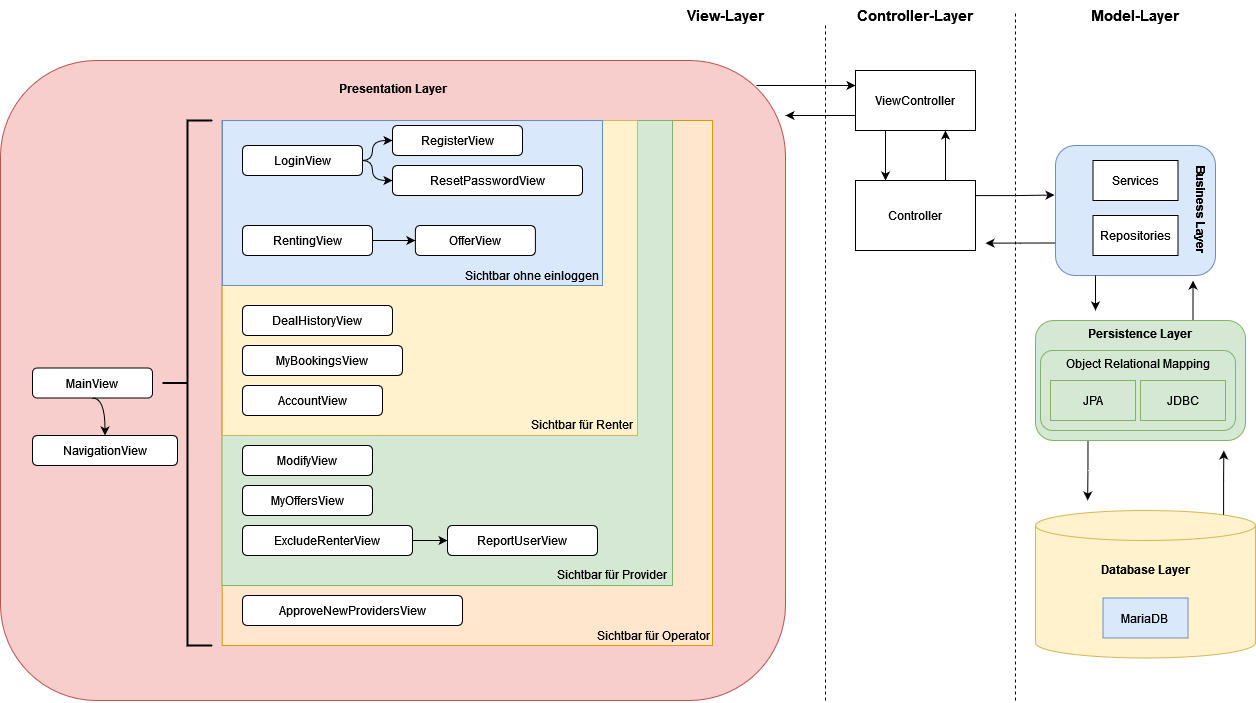
\includegraphics[width=15cm]{resources/images/architecture.drawio.png}
	\caption{General Architecture of SWTcamper}
	\label{fig:architecture}
\end{figure}

\subsubsection{Layered MVC in general}
The Model-View-Controller pattern is an architecture or design pattern that offers flexible program design, makes it easier to change or expand it later, and allows the individual components to be reused.
Applications designed according to the principles of MVC consist of three interchangeable components:

\begin{itemize}
	\item \textbf{The model} consists of several model classes. Each represents a basic entity within the data structure used. They also provide basic data operations that are not necessarily part of the basic program logic. This includes, for example, the individual entities on the basis of which the application runs, or the services that provide the necessary values from the database and can already process them to the necessary degree.
	
	\item \textbf{View} classes provide the graphical user interface. The model classes provide the displayed data, but there is no direct connection between the two program parts. The controller informs the components of the surface display about changes to the model and they adjust the displayed content if necessary.
	
	\item \textbf{The controller} classes act as a connector between view and model components. The view forwards user actions to the controller, which executes the underlying program logic. If necessary, the logic informs individual views about changes to the model in order to enable an appropriate reaction to them.
\end{itemize}

\subsubsection{JavaFX (view)}
JavaFX is a framework for creating cross-platform Java applications. With FXML, it enables a declarative description of graphical user interfaces based on XML. The Scene Builder is a graphical tool that simplifies the creation of FXML files. In addition, web technologies such as CSS can also be used for the design by embedding them in the FXML code. \\
View controllers are the controllers of the individual views, which not only take care of event handling, but also request and forward data from the 'real' controllers. \\
We used all of these functions as part of this project. The views were only generated programmatically for dynamic program parts, like the list of available displays or the operator dashboard.

\subsubsection{Spring boot (view, controller, model)}
Spring Boot is an open source framework that offers many functionalities for developing a standalone application. It simplifies the software development process by reducing complexity and providing a clear structure. Especially in contrast to classic Spring applications, where several XML configuration files had to be edited, Spring Boot offers a quick creation of a new project. \\
In order for the framework to know how to deal with each class, there are annotations that allow Spring Boot to create the necessary environment for the classes. An example of this is the \textit{@Service} annotation, which is placed above each of our service classes, or \textit{@Component}, which is used above each controller.

\subsubsection{JPA (model)}
The \textit{Jakarta Persistence API} is an interface for Java applications that simplifies the assignment and transfer of objects to database entries. It simplifies solving the object-relational mapping problem of storing run-time objects of a Java application across a single session (persistence). Various settings can be made through annotations in the entity classes in order to implement the desired database schema automatically.

\subsubsection{Docker (model)}
Docker is open source software that allows us to run applications in a virtual container environment. Docker simplifies the deployment of applications because containers that contain all the necessary packages can be easily transported and installed as files. Containers ensure the separation and management of the resources used on a computer. We used Docker to run our \textit{MariaDB} database in it.

\subsubsection{MariaDB (model)}
MariaDB is an open-source relational database-system and a fork of \textit{MySQL}. We used it to store our data consistently. MariaDB can be used by its own Docker image.

\subsection{Design Implementation}
In order to understand which components we need for the application and how best to proceed, we created a use case diagram (fig. \ref{fig:use-case-diagram}) and an ER diagram (fig. \ref{fig:er-diagram}) in Sprint 0, which have changed over the course of the project.

\begin{figure}[h]
	\centering
	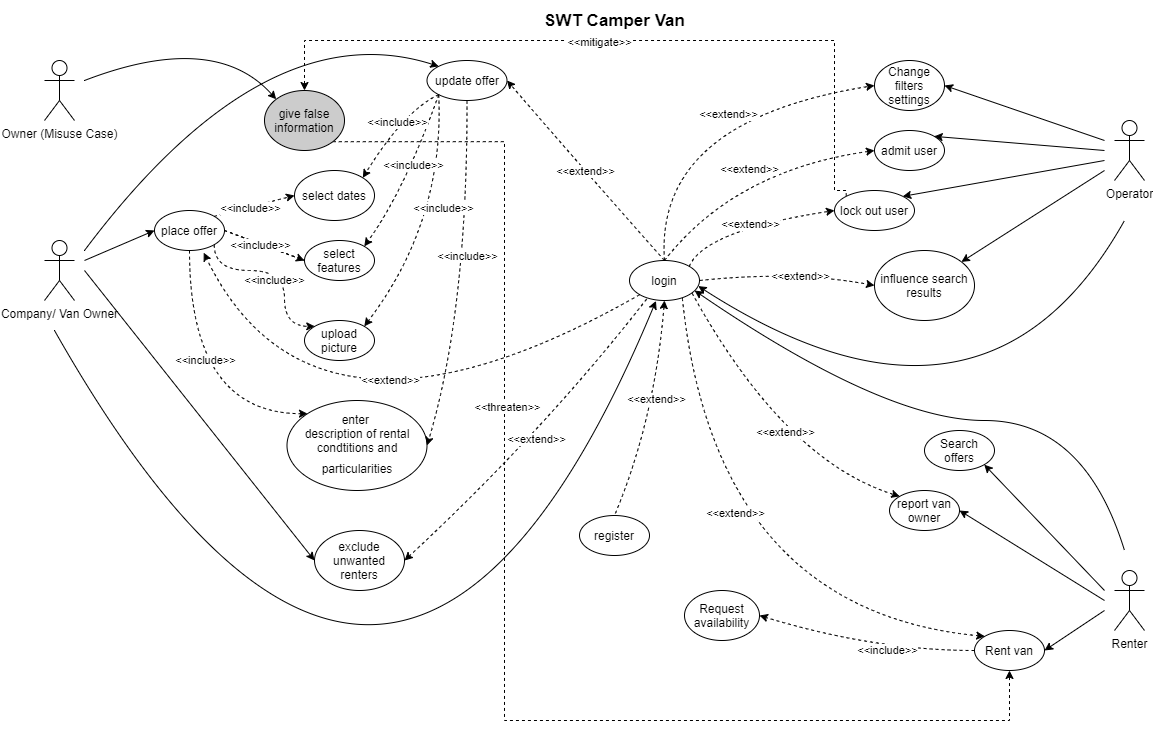
\includegraphics[width=12cm]{resources/images/use-case-diagram.png}
	\caption{Use Case Diagram}
	\label{fig:use-case-diagram}
\end{figure}

\paragraph{Basic Structure}
The heart of SWTcamper is the \textit{MainView} and its associated view controller, which is called directly from \textit{App.java} (starting point for JavaFX applications) when the program starts. Via imports, it contains all other FXML views that are added or removed via the controller depending on the \textit{NavigationViewController}. (trying to show in fig. \ref{fig:architecture}) When the program starts, the \textit{RentingView} is loaded first via the \textit{changeView()} method, which contains all available displays. To do this, the \textit{AnchorPane} 'mainStage' in the \textit{MainView} is first completely emptied and then filled with the \textit{RentingView} mentioned. If the user now presses a button in the \textit{NavigationView} (buttons are displayed depending on the \textit{UserRole} (also taken from fig. \ref{fig:architecture})), the \textit{MainViewController} is instructed via its view controller to repeat the same procedure for the newly selected view. In order to differentiate between the views, a suitable string must be passed to the \textit{changeView()} method (e.g. 'home' for the \textit{RentingView} or 'history' for the \textit{DealHistoryView}). Since all view controllers are already initialized when the program starts, all other view controllers must also be imported into the \textit{MainViewController} so that a reload method can be called for each one individually.

\subsection{Class diagrams}
We made a class diagram in the first sprints. Since our classes have changed since then, we wanted to include an automatically generated class diagram at this point; However, since this is much too big, we tried to split it up into its most important classes and integrate them separately. The diagrams can be viewed in the Additional Material (fig. \ref{fig:cd:controller-services} and fig. \ref{fig:cd:entities} (note: for the sake of clarity we missed out attributes and methods, but at least for the entities these can be seen in our ER-diagram (fig. \ref{fig:er-diagram}))).

\subsection{Data model \& Design decisions}
In order to get an overview of the entities to be implemented and how they interact, we created an ER-diagram at the beginning of Sprint 0 (fig. \ref{fig:er-diagram_draft}), which only changed slightly over the course of the project has (fig. \ref{fig:er-diagram}). In this chapter we present our entities and their structures.

\paragraph{Booking}
The Booking class is required to bind a user to an offer. To do this, it has an ID that is automatically generated by the database (through the \textit{@Id} and \textit{@GeneratedValue} annotations), a user who wants to rent the associated offer, the offer itself, a start date and an end date. Furthermore, there are the two boolean fields \textit{active} and \textit{rejected}. A booking is created with \textit{active = false} and remains inactive until accepted; if it is rejected, the field \textit{rejected}, which was also created with \textit{false}, is set to \textit{true}. The combination of these two values is used at several points in the application to determine states:

\begin{table}[h]
	\centering
    \caption{\label{tab:booking-variables}Deriving logic from combination of variables in Booking class}

	\begin{tabular}{|c|c|c|c|}
		\hline
		&  & \multicolumn{2}{c|}{active} \\
		\hline
		&  & true & false \\
		\hline
		rejected & true & \begin{tabular}[c]{@{}c@{}}Offer ended early,\\gets listed in offer history\end{tabular} & / \\
		\hline
		& false & \begin{tabular}[c]{@{}c@{}}Offer can not get modified\\or deleted\end{tabular} & \begin{tabular}[c]{@{}c@{}}Provider sees offer as\\``New request for offer''\\(not yet in offer history)\end{tabular} \\
		\hline
	\end{tabular}
\end{table}

\paragraph{Filter}
The Filter class is the only entity class in SWTcamper that is not stored in the database. It contains all the fields from \textit{Offer} and \textit{Vehicle} that are required for a good search. When the search is started, a new filter instance is created and the necessary fields are set. This instance is then passed to the \textit{OfferController}, which uses it to filter the list of all offers and returns a new list of offers that match the filter instance.

\paragraph{LoggingMessage}
Logging messages are generated by almost all services and are required to be able to track events. A list of logging messages can be viewed as an operator via the \textit{AccountView} and downloaded as a log file. Since all logging messages that occur are also stored in the database, each has a unique and automatically generated ID and a time stamp for which it was created. The enum \textit{loggingLevel} indicates how important the logging message is (INFO, WARNING, ERROR) and there is also a message so that the viewer knows what it is about.

\paragraph{Offer}
The offer class was implemented first in SWTcamper together with the vehicle class. In the course of development, however, it was expanded and improved. It is needed to display offers - one of the basics of SWTcamper. Objects of this class have an ID automatically generated by the database, a user who created the offer, title, pick-up location, contact details via which the creator would like to be reached, special features of the offer (such as things that are not already covered by SWTcamper ) and a price. Via \textit{active} the creator can specify whether the offer should be publicly listed and if \textit{promoted} is \textit{true} the offer will be highlighted in the list; this function can only be changed by operators, but is visible to all users. Of course, each offer also contains a permanently associated vehicle object with all its values and lists for blocked dates for which the offer cannot be booked, non-overlapping bookings and rentalConditions, with which the creator specifies conditions to which the renter adheres has to hold. \\
The \textit{offeredObjectType} field is no longer used in our version of SWTcamper; however, it would be possible to extend the application here.

\paragraph{Picture}
Originally it was planned that the images stored in SWTcamper for the vehicles would be completely loaded into the database; however, there were many problems finding the right data type and there were many errors that the database could not store objects of this size. So next we switched to storing a list of paths in the Vehicle object. However, this list was also too long for the database from around three images onwards. \\
As a solution, we have therefore created our own repository for the images. In addition to the obligatory ID, each entry contains the path to the image and the ID of the vehicle to which it is to be assigned. \\
Unfortunately, this approach means that images can only be stored locally and do not work in a distributed system. However, since our application only had the requirement to run locally anyway, that was fine for this framework.

\paragraph{User}
In addition to an automatically generated ID, the User class also has attributes for the username, first and last name, email address, telephone number and password. The \textit{userRole} attribute indicates which role the user assumes when using the application and which authorizations he has as a result (cf. view illustration in fig. \ref{fig:architecture}). Related to this there is also the attribute \textit{enabled}, which is only set to \textit{false} when a user registers as a new provider, since it was a requirement that these people should first be checked before they can create new offers. As long as a user has the role of provider and \textit{enabled} is set to \textit{false}, he has the same powers and options as the \textit{userRole} Renter. \\
Another boolean field is \textit{locked}, which is required to globally block a user; its application options are therefore severely limited. In contrast to this possibility, which can only be carried out by an operator, there is also one for providers with which other users can be excluded from their offers. To do this, User objects use a list \textit{excludedRenters}, in which the IDs of the users to be excluded are stored.

\paragraph{UserReport}
UserReports are required so that one user (as of UserRole Provider) can report another. A submitted UserReport is then stored in the database (again has an automatically generated ID) and has an \textit{active} boolean field set to \textit{true} until the report is processed (\textit{accepted} or \textit{rejected}) by an operator. In order to make it easier for the decisive operator to make his decision, each UserReport contains both the username of the reporter and the reported person and a message explaining why the reporter submitted the report.

\paragraph{Vehicle}
Just like the offer class, the class for the vehicles themselves plays a very central role, which is why it was implemented first. It contains very rudimentary attributes to represent the vehicles offered; in addition to the automatically generated ID, this includes the brand, model, year of construction, length, width and height, the type of connection, the number of seats and the number of beds. Simple boolean variables were used to describe whether the vehicle has a roof tent, roof rack, bike rack, shower, toilet, kitchen unit or refrigerator. There are also separate enumerations for the type of vehicle and the type of fuel.

\subsection{Design Principles}

\subsubsection{General Principles}

\paragraph{Hide information}
Similar to what is explained in SOLID's Open-Closed-Principle (\ref{subsec:solid:ocp}), we have applied the 'public' and 'private' access modifiers as far as possible, so that the classes are encapsulated as much as possible. However, we really only used 'public' and 'private' and neglected e.g. 'protected', which only allows visibility within the current package. Implementing this would improve the quality of the software and could well be done in another sprint.

\paragraph{Loose Coupling}
The parts of SWTcamper's Model-, View- and Controller components are clearly seperated from each other and communicate only through interfaces.

\paragraph{Program to an interface, not an implementation}
In SWTcamper we have interfaces for our repositories for the database, for our backend controllers and for our entities. Since we didn't apply this principle from the beginning, but relatively late, we didn't build the interfaces for the entities into the rest of the code, so that they are instantiated directly and not via their interfaces (which would need casts to normal classes anyway). This task would be a good fit for another sprint and shouldn't take much time. In the meantime, the interfaces still represent a kind of 'security template'. For the first two class groups, however, we have applied it according to the principle.

\paragraph{High Cohesion}
This is pretty similar to SOLID's SRP (\ref{subsec:solid:srp}); as mentioned there our classes mostly have only one purpose. Improvments could be made in the MainViewController which also includes the database scanner.

\paragraph{Encapsulate Logic}
This principle was implemented in our application primarily by the fact that the frontend controllers do not have direct access to the backend controllers, but only to the methods from the backend controllers' interfaces.

\subsubsection{SOLID Design Principles}

\paragraph{Single-Responsibility-Principle}
\label{subsec:solid:srp}
For SWTcamper we implemented contract classes and DTO objects. Through this
feature we are able to display the objects of the database with additional information that
can be useful to the user without modifying the objects themselves. Real changes to the objects
are only carried out by saving, deleting or updating operations to ensure that we comply with them
the principle of individual responsibility. \\
Otherwise, our classes mostly have only one purpose. An exception is the MainViewController, which, in addition to managing the other view controllers, also scans the database for changes every second.

\paragraph{Open-Closed-Principle}
\label{subsec:solid:ocp}
By using the MVC pattern it is possible to exchange the frontend without changing the backend. Replacing the database with another one wouldn't be difficult either, as long as JPA is still able to map the objects correctly. This is made even easier by the fact that our database is made available in a container using Docker, which is easier to exchange than without. \\
Furthermore, it would be possible to extend our existing interfaces; however, this was not explicitly valued during development. Instead, we have kept as much internals as possible private, so that classes are encapsulated from the outside as much as possible, which has worked almost completely with a few exceptions.

\paragraph{Liskov's Substitution-, Interface-Segregation- and Dependency-Inversion Principles}
Since we did not go into design principles too much when planning, we did not find any examples for these principles in our application. It is possible that SWTcamper is less suitable for this in its current form. \\
A possible implementation of Liskov's substitution principle would be to implement the IUser interface in the three different user classes Renter, Provider and Operator, instead of implementing it via an enumeration of UserRoles as we did. That would certainly be a point that could be improved in future sprints.

\subsection{Design Patterns}

\subsubsection{Behavioral patterns}

\paragraph{Observer Pattern}
\label{subsec:observer-pattern}
We would have liked to have used this pattern to implement the notifications in such a way that the database automatically sends notifications to all observers (push notification). Unfortunately, we found that MariaDB does not support such functionality. But it was possible to implement a so-called entity listener via Spring Boot annotations; This caused a thread to be started in the background, which checked for changes to the respective entity objects at regular intervals and executed the desired functionality if there was a change. However, inconveniently, in our application this caused the notification dots (the objects that the thread should change when an entity changes) to flicker in the navigation bar, so we decided to implement such a scanner ourselves, which actually worked better: \\
To do this, we implemented the \textit{listenForDataBaseChanges()} method in the \textit{MainViewController}, which fetches the necessary objects from the database and saves them in local variables. After the next fetch, it then compares these variables with the new data and executes the corresponding functionalities if the two data sets are different differentiate. So that this is possible at regular intervals, the method was provided with \textit{@Scheduled(fixedDelay = 1000)}, which also starts a new thread in which, in contrast to the first implementation, the time intervals can be controlled. This implementation also corresponds to the pull notification of the observer pattern.

Furthermore, we used properties in many places in the application and either bound them to others or set EventListeners on them so that dependencies adjust automatically without having to trigger the functionality separately. \\
The (forced by JavaFX) use of observable lists is also to be assigned to the observer pattern, since changes in the lists automatically cause a change in the objects in which they are used.

\subsubsection{Creational patterns}

\paragraph{Singleton Pattern}
Since the structure of SWTcamper is designed in such a way that the \textit{MainView} holds all other views (cf. fig. \ref{fig:architecture}), only one object is created at the start of the \textit{MainViewController} and the \textit{NavigationViewController}, which are permanently displayed and their contents are only change. However, both are also referenced in other view controllers using Spring Boot's \textit{@Autowired}, so at this point we are not 100 percent sure how the framework handles these classes exactly. \\
It would also have been nice to have the database scanner explained in section \ref{subsec:observer-pattern} in its own class, so that it would only be instantiated once - independent of the \textit{MainViewController}. However, it can be assumed that this will only happen once.

\paragraph{Factory Method}
We didn't use this method explicitly, but because we use the Spring Framework and provide many similar classes with the same annotations (\textit{@Component}, \textit{@Service}, \textit{@Entity}, \textit{@Repository}), they use the same interfaces and therefore also have the same standard methods , such as \textit{initialize()}. \\
An explicit implementation might be possible with the ViewControllers; Due to the component-based structure of the application, however, our classes differ so much that sharing interfaces is of little use.

\subsubsection{Structural patterns}

\paragraph{Decorator Pattern}
Initially, to create a new ad and to edit an ad, we had two different views and controllers. However, since the two functionalities are so similar, we have combined them in a view (and thus a controller) \textit{ModifyView}. There is a boolean variable to distinguish between creating a new ad or editing an existing one. The decorator pattern could have been used here, which would extend the class with additional functionality at runtime. However, it is questionable whether this would bring a real advantage given the size of our application and the class.

\paragraph{Pipes and Filters}
We used functional programming in SWTcamper in several places, especially when processing lists (e.g. for filters), and lined up the methods so that the output of the last processing step was always the input for the next.

\subsection{Summary}
In SWTcamper we have applied many of the design principles we are familiar with - partly consciously and partly unconsciously. In some cases, we only implemented them when writing this report, after hearing from them again. Overall, we could definitely implement more with more time and also with higher accuracy. In addition, it would also be good in the future to go into the principles more at the beginning of the architecture and not only later on, but in retrospect we neglected that a bit too much.

% % %
\cleardoublepage
\section{Realisation}
\label{sec:realization}

\begin{itemize}
    
    \item \textbf{Sprint 0:} In sprint 0, we conducted the Blastoff activities, which produced several artifacts including a Use Case Diagram, and held a User Story workshop. Based on these, we devised a rough project plan, which was discarded after feedback from the client in the sprint review meeting. Instead of spreading the User Stories numerically sorted over the coming sprints, the client advised us to choose User Stories which will present something of value to the customer, and prioritize those which require a lot of feedback.

    \item \textbf{Sprint 1:} In sprint 1 we planned to apply the clients feedback on our artifacts and to realize the first functionalities. We created an extensive prototype and began with the implementation of the lifecycle of the offer object, namely creation and updating.

    \item \textbf{Sprint 2:} The vision for sprint 2 was to, after we implemented the basic functionalities of an offer, to take the next step and make it possible to filter/search offers. Another goal was to begin the implementation of the login and registration functionality, so that we could start realizing user roles in the sprints to come.

    \item \textbf{Sprint 3:} The goal for sprint 3 was to continue our intention to start the realization of user roles and their aspects. We planned to implement the handling of bookings from the renters and the providers perspective.

    \item \textbf{Sprint 4:} Aside from having to catch up with tasks left over from sprint 3, sprint 4 was dedicated to user management, namely the ability of providers to exclude renters, and the ability of operators to block, accept or promote/degrade users. Also planned was to increase our efforts to assure software quality through testing code and the prototype.

    \item \textbf{Sprint 5:} Sprint 5, the final sprint, was dedicated to extensive unit and integration testing of the core parts of the application, as well as fixing any open issues, if possible. The teams focus also lay on realizing a good last increment of the application to show the customer in the final presentation.

\end{itemize}

% % %
\cleardoublepage
\subsection{Sprint No.~1}
\emph{\textbf{Approximate expected report length:} 2--3 pages of text}

\subsubsection{Sprint Planning}
\usepackage{booktabs}\paragraph{Goal}
Our officially stated goal for this sprint was:\\
\textit{In the next two weeks ("Sprint 1"), you should correct the artifacts from Sprint 0 with respect to the feedback from Prof. Lüttgen and start with implementing the first few User Stories. To do this into the xTasks project, the team first (?) needs to clean it up.}

But with the experience we have after sprint 5 we would rather formulate it like this (shorter and on point):\\
\textit{Implement the possibility for a provider to place new and update existing offers such that they can be seen in the application.}

% \paragraph{User Stories we worked on in this sprint}

% \heading{User Story 02: Place offer (Size: M, Sprint 1)}

% As a Provider,\\
% I want to place an offer,\\
% so that my vehicles can be booked by renters.

% The story is done, when
% \begin{itemize}
%     \item it is possible to enter info about a vehicle (images, features, dates when it is available, description of rental conditions, particularities) into a form, which will then be considered an offer by the system.
%     \item it is possible for renters to find my offer via the search function.
%     \item it is impossible to offer the same vehicle multiple times.
%     \item the offer/vehicle is entered into the database.
%     \item each offer shall have obligatory information. If this information is not filled-in provider cannot create the offer.
% \end{itemize}


% \heading{User Story 03: Update offer (/ Delete) (Size: M, Sprint 1)}

% As a Provider,\\
% I want to update an existing offer,\\
% so that the information is up to date.

% The story is done, when
% \begin{itemize}
%     \item the provider can enter an “Edit”-Mode by clicking a button on the offer screen, which is only shown to provider accounts.
%     \item the button is only shown on offers belonging to the respective provider.
%     \item after editing the offer is finished, the database entry of the offer gets updated.
%     \item providers can access the list of their offers.
%     \item The provider can delete the offer.
% \end{itemize}


\paragraph{Tasks that have been worked on \newline \newline}

\begin{tabular}{|l|c|c|}
	\hline
	\href{https://gitlab.rz.uni-bamberg.de/swt/teaching/2021-ws/swt-swl-b/group-a/-/issues/28}{All-Offer View} & User Story 3 & Patrick \\
	\hline
	\href{https://gitlab.rz.uni-bamberg.de/swt/teaching/2021-ws/swt-swl-b/group-a/-/issues/27}{Update vehicle Database Connector} & User Story 3 & Sabir \\
	\hline
	\href{https://gitlab.rz.uni-bamberg.de/swt/teaching/2021-ws/swt-swl-b/group-a/-/issues/24}{Database Connector} & User Story 2 & Aaron \\
	\hline
	\href{https://gitlab.rz.uni-bamberg.de/swt/teaching/2021-ws/swt-swl-b/group-a/-/issues/23}{View Controller} & User Story 2 & Oleksandr \\
	\hline
	\href{https://gitlab.rz.uni-bamberg.de/swt/teaching/2021-ws/swt-swl-b/group-a/-/issues/41}{Create}/\href{https://gitlab.rz.uni-bamberg.de/swt/teaching/2021-ws/swt-swl-b/group-a/-/issues/34}{Update}/\href{https://gitlab.rz.uni-bamberg.de/swt/teaching/2021-ws/swt-swl-b/group-a/-/issues/35}{Delete} Offer & User Story 3 & Patrick/ Thomas \\
	\hline
	\href{https://gitlab.rz.uni-bamberg.de/swt/teaching/2021-ws/swt-swl-b/group-a/-/issues/37}{Lo-Fi Prototype} &  & Oleksandr \\
	\hline
	\href{https://gitlab.rz.uni-bamberg.de/swt/teaching/2021-ws/swt-swl-b/group-a/-/issues/19}{Prioritize User Stories \& Issues} &  & Melissa \\
	\hline
	\href{https://gitlab.rz.uni-bamberg.de/swt/teaching/2021-ws/swt-swl-b/group-a/-/issues/25}{Update Vehicle View} & User Story 3 & Thomas \\
	\hline
	\href{https://gitlab.rz.uni-bamberg.de/swt/teaching/2021-ws/swt-swl-b/group-a/-/issues/26}{Update Vehicle View Controller} & User Story 3 & Thomas \\
	\hline
	\href{https://gitlab.rz.uni-bamberg.de/swt/teaching/2021-ws/swt-swl-b/group-a/-/issues/21}{Vehicle Controller} & User Story 2 & Aaron \\
	\hline
	\href{https://gitlab.rz.uni-bamberg.de/swt/teaching/2021-ws/swt-swl-b/group-a/-/issues/20}{Vehicle class} & User Story 2 & Melissa \\
	\hline
	\href{https://gitlab.rz.uni-bamberg.de/swt/teaching/2021-ws/swt-swl-b/group-a/-/issues/30}{Offer class} & User Story 2 & Melissa \\
	\hline
	\href{https://gitlab.rz.uni-bamberg.de/swt/teaching/2021-ws/swt-swl-b/group-a/-/issues/22}{View Place Offer} & User Story 2 & Patrick \\
	\hline
	\href{https://gitlab.rz.uni-bamberg.de/swt/teaching/2021-ws/swt-swl-b/group-a/-/issues/17}{Fix Architecture Diagram} &  & Patrick \\
	\hline
	\href{https://gitlab.rz.uni-bamberg.de/swt/teaching/2021-ws/swt-swl-b/group-a/-/issues/10}{Project Plan} &  & Melissa \\
	\hline
	\href{https://gitlab.rz.uni-bamberg.de/swt/teaching/2021-ws/swt-swl-b/group-a/-/issues/31}{Clear Project to Skeleton} &  & Sabir \\
	\hline
	\href{https://gitlab.rz.uni-bamberg.de/swt/teaching/2021-ws/swt-swl-b/group-a/-/issues/16}{Fix Use Case Diagram} &  & Aaron \\
	\hline
	\href{https://gitlab.rz.uni-bamberg.de/swt/teaching/2021-ws/swt-swl-b/group-a/-/issues/32}{Create dev + production branch} &  & Sabir \\
	\hline
	\href{https://gitlab.rz.uni-bamberg.de/swt/teaching/2021-ws/swt-swl-b/group-a/-/issues/15}{Acceptance Criteria \& INVEST Review} &  & Oleksandr \\
	\hline
	\href{https://gitlab.rz.uni-bamberg.de/swt/teaching/2021-ws/swt-swl-b/group-a/-/issues/36}{Review Acceptance Criteria} &  & Thomas \\
	\hline
\end{tabular}


\subsubsection{Noteworthy Development Aspects}
In this sprint we have broken down the functionalities far too much into their individual parts (e.g. each controller or view individually named); this meant that team members could not work independently on their issues because they had to wait for others who had the same problem themselves. This 'deadlock-like' condition was also an important part of our retrospective to avoid this mistake in future sprints. \\
You can also see that in addition to the user stories, work was also carried out on issues that were either improvements from Sprint 0 or that are important for the project itself (such as the design of a prototype or the redesign of our project plan). \\
The move from the \textit{xTasks} skeleton to \textit{swtcamper}, as already mentioned in the (now old) Sprint Goal, has also been processed. \\
Unfortunately, the order in which we carried out the merge requests afterwards led to serious problems that we will also take with us into the next sprint and work on there. The better solution probably would have been to carry out all merge requests first and only then to move to \textit{swtcamper}. We did it the other way around.

\paragraph{Problems that occured and how we solved them}

\begin{itemize}
    \item Docker did not run on Windows 7 $\rightarrow$ the affected team member worked on other tasks first and bought a new PC by now
    \item \textit{MainController} cannot be implemented without the other Controllers $\rightarrow$ good and early conversation in the team made it possible anyway
    \item IntelliJ had problems with JavaFX $\rightarrow$ the help desk found out that this particular error came from the use of a wrong
    sub folder
    \item Correct usage of branches $\rightarrow$ a team member gave the others a quick introduction into Gitlab's 'Create Merge Request' from within the issue itself and also showed how to work on Merge Requests
    \item how to upload pictures and save pictures since the database complained about the size of the stored object? $\rightarrow$ after consultation with the client it was ok to not upload the pictures but just save their paths
    \item IntelliJ shows Class as not existent - even if it is $\rightarrow$ This problem is not fixed until today but since it's only from IntelliJ's linter it works anyway, but stays annoying
    \item 'Merge Hell' – we should have done 'clear codebase to skeleton' after merging everything, not started with everything else and merge it into new \textit{/swtcamper/} $\rightarrow$ As already stated, this problem came with us into Sprint 2 and had to be worked on further, but we could solve it and avoided it from there on mostly
\end{itemize}

\subsubsection{Sprint Review}
\paragraph{Describe the product increment produced in this sprint}
When starting the application, only two of the visible tabs can be clicked on and used: on the
one hand, "Login" and on the other hand, "Rent a Camper". The latter has not yet been
implemented and the login is implemented more demonstratively than functional: there is
only one "Login" button which, after clicking on it, activates the other tabs "My Offers" and
"Place Offer". All offers that have already been placed can be viewed in a list under “My
Offers”. Above that are the buttons “Place Offer”, “View Offer”, “Update Offer” and “Delete
Offer”.
Via “Place Offer” the user is automatically taken to the tab of the same name. Here he can
enter information on the offer (title, price per day, location, availability) and on the vehicle
itself (vehicle type, make, model, year of construction). For the latter, the user can also select
features and upload images.
At this point in time, only the title and price per day can be saved in the increment.
Using the “Place Offer” button, the user can then return to “My Offers” where the new offer
is listed accordingly.
To change the offer, you can click on the "Update Offer" button, which activates the tab of
the same name and takes you to it. The same form can be seen here as on "Place Offer", only
this time the relevant fields are already filled out and ready to be changed. Once this is done,
the "Update Offer" button can be clicked, which brings the user back to "My Offers". The
“Update Offer” tab is now also deactivated again.
Via the “View Offer” button, the user receives an info alert at this point in time, in which the
relevant information (including the ID from the database) can be seen. The same function is
also hidden behind a double-click on an offer.
With the last button “Delete Offer”, the selected offer is deleted from the database after a
request in the form of a warning alert.
If no offer is selected and the user presses one of the buttons, he will also receive an alert
with the instruction to select an offer first.

\paragraph{Compare the achieved increment with the sprint goal and the user stories that were chosen for this sprint}
The sprint goal was achieved (for the most part):
- A new offer can be created (and saved in the database), displayed in a list, updated and
deleted.
- In addition, our Blast Off was updated (w.r.t. the feedback we got).
- The only thing that has not yet been fully achieved is the move to swtcamper, or
already, but has not yet been fully merged with the functionalities.

\paragraph{Give a brief summary on your team's retrospective, including changes to the product backlog}
We learned from the customer that our menu navigation in the prototype is still too
complicated (too few links), that a user should be able to have several roles at the same time
and that an offer should not be deletable if it is already rented out (or that the User is
communicated somehow).
We learned from the client that our sprint goal should direct more joy to the customer and
that quality assurance is not only possible via code, but can and should also be applied
through tests / methods, such as usability testing, before implementation.



% % %
\cleardoublepage
\subsection{Sprint No.~2}
\paragraph{Primary textual contributors.}
\mbox{}\\\emph{Aaron Hißting}

\subsubsection{Sprint Planning}
\paragraph{Goal} \\
The goal of sprint 2 was to implement two core parts of our application: The search/filter functionality, which would give users the means to find vehicles meeting their needs as precise as possible, and the Registration/Login functionality, which would allow users to create a user account and specify which role they would like to assume (at this point in time we differentiated between a basic user, called User, and the Operator. This was changed to renter, provider, operator after consultation with the customer). To achieve this goal, we had to work on User Story 01: Registration/Login and User Story 06: Filter. Following is a list of all User Stories and tasks we worked on in this sprint: \\

\begin{table}[h]
    \centering
    \caption{User Stories and tasks worked on in sprint 2}
\begin{tabular}{|l|c|c|}
    \hline
    \href{https://gitlab.rz.uni-bamberg.de/swt/teaching/2021-ws/swt-swl-b/group-a/-/issues/56}{Implement search functionality} & User Story 6 & Thomas, Patrick \\
    \hline
    \href{https://gitlab.rz.uni-bamberg.de/swt/teaching/2021-ws/swt-swl-b/group-a/-/issues/55}{Implement registration/login} & User Story 1 & Melissa, Oleksandr \\
    \hline
    \href{https://gitlab.rz.uni-bamberg.de/swt/teaching/2021-ws/swt-swl-b/group-a/-/issues/58}{Implement mandatory offer fields} & User Story 2 & Patrick \\
    \hline
    \href{https://gitlab.rz.uni-bamberg.de/swt/teaching/2021-ws/swt-swl-b/group-a/-/issues/48}{Implement full CRUD functionality Offer} &  User Story 2 & Aaron, Sabir \\
    \hline
    \href{https://gitlab.rz.uni-bamberg.de/swt/teaching/2021-ws/swt-swl-b/group-a/-/issues/49}{Offer Lifecycle / State Machine Diagram} & User Story 2 & Aaron \\
    \hline
    \href{https://gitlab.rz.uni-bamberg.de/swt/teaching/2021-ws/swt-swl-b/group-a/-/issues/52}{Finalize offer} & User Story 2 & Aaron, Patrick \\
    \hline
    \href{https://gitlab.rz.uni-bamberg.de/swt/teaching/2021-ws/swt-swl-b/group-a/-/issues/59}{Place Offer View überarbeiten} & User Story 2 & Thomas \\
    \hline
    \href{https://gitlab.rz.uni-bamberg.de/swt/teaching/2021-ws/swt-swl-b/group-a/-/issues/60}{Implement missing Offer fields} & User Story 2 & Thomas \\
    \hline
    \href{https://gitlab.rz.uni-bamberg.de/swt/teaching/2021-ws/swt-swl-b/group-a/-/issues/61}{Adapt MyOfferView} & User Story 2 & Aaron, Thomas \\
    \hline
    \href{https://gitlab.rz.uni-bamberg.de/swt/teaching/2021-ws/swt-swl-b/group-a/-/issues/50}{Fix dev branch} & & Thomas \\
    \hline
    \href{https://gitlab.rz.uni-bamberg.de/swt/teaching/2021-ws/swt-swl-b/group-a/-/issues/51}{Set entity structure} & & Melissa, Aaron, Patrick \\
    \hline
    \href{https://gitlab.rz.uni-bamberg.de/swt/teaching/2021-ws/swt-swl-b/group-a/-/issues/53}{Adjust prototype} & & Oleksandr, Sabir \\
    \hline
    \href{https://gitlab.rz.uni-bamberg.de/swt/teaching/2021-ws/swt-swl-b/group-a/-/issues/54}{Implement Unit Tests for Offerservice} & & Melissa, Sabir \\
    \hline
    \href{https://gitlab.rz.uni-bamberg.de/swt/teaching/2021-ws/swt-swl-b/group-a/-/issues/57}{Implement navigation} & & Thomas, Sabir \\
    \hline
\end{tabular}
\end{table}


\subsubsection{Noteworthy Development Aspects}
After a somewhat chaotic sprint 1, we decided to revise our development approach. We identified several issues:

\begin{itemize}
    \item \textbf{Not enough planning:}
    \begin{itemize}
        \item \textbf{Solution:} When creating an issue/task during/after the product backlog meeting (our name for a preliminary sprint planning meeting which was held right after the sprint review meetings by two team members, and during which we went over the meeting notes of the last review and created all foreseeable tasks), think about who would be suited best to work on it. By doing this, the process of allocating tasks to team members during the following sprint planning meeting could be sped up.
    \end{itemize}
    \item \textbf{Difficulties keeping an overview over the current state of the application:}
    \begin{itemize}
        \item \textbf{Solution:} We decided to be stricter in our handling of issues, we made it mandatory to include a due date, a user story/milestone, a brief description if sensible and to assign a team member as soon as the issue is moved from product backlog to sprint backlog. In addition to that, we emphasized that every team member is responsible for updating their issues when necessary and to keep an eye on the overall orderliness of the issues board.
    \end{itemize}
    \item \textbf{Due to insufficient coding experience of most team members, code quality was poor:}
    \begin{itemize}
        \item \textbf{Solution:} We decided to assign two team members to any non-trivial tasks. By using the pair programming technique, we assured that two team members write and think about a part of the application at the same time. To further utilize this technique, we assigned not just any two team members, but, where possible and sensible, team members from different “areas of expertise” (e.g., frontend and backend, or, when writing interfaces, two team members from each “side” of the interface, i.e. one from each part of the application the interface is supposed to “connect”. An example would be). In addition to that, we decided to emphasize the importance of thoroughly reviewing code, either when asked to do so or when handling merge requests. We made sure to never let someone who worked on the branch to be merged handle the merge request, but a third person with “fresh eyes”.
    \end{itemize}
    \item Insufficient experience with the technology used (e.g., git, Docker, Spring Boot, working with databases)
    \begin{itemize}
        \item \textbf{Solution:} We emphasized using the “Manual” page in the GitLab wiki, which was created to gather helpful tips and commands, and even short tutorials on common use cases (e.g., GitLab markdown tags, additions to the docker-compose commands)
    \end{itemize}
\end{itemize}

Artifacts produced in sprint 2 were .fxml files for each view necessary to fulfill our sprint goal (rentingView, loginView, registrationView, resetPasswordView), as well as navigationView.fxml, and the respective ViewController classes. In addition, we updated our prototype to now include the sprint goal functionalities and feedback we received in the last sprint review meeting from the customer: A new navigation sidebar so users can quickly and always access all subsections of the application, with icons instead of written out menu items, in order to keep the sidebar slim and to make (at least the menu) language independent. The sidebar can be expanded to show the actual menu item names. The layout was changed to a widescreen format, a FAQ section was added, as well as a deal history section to record current and previous bookings, and a screen demonstrating the functionality to add custom vehicle features when creating an offer.

As we added the actual offer attributes to the offer class, we realized that the lifecycle of offers is more complex than we thought, so an offer lifecycle diagram was created. During creation of the diagram, we discovered several questions we hadn’t asked ourselves before, e.g. what happens upon deletion (whether the offer is actually deleted depends on its active/inactive status), or how we should handle the availability of offered vehicles (instead of a simple Boolean (which in retrospect didn’t make sense as an offer, as we implemented it, cannot be available or unavailable as a whole, only for periods of time) we started to think about the concept of a booking object).

Obstacles we encountered in this sprint were in part of organizational nature, i.e., team members, due to personal reasons, not being available as much as planned. Because of this the pair programming approach was abandoned for the task “Implement search functionality”, which we compensated for by assigning one of the more experienced team members. Difficulties with git kept a team member from working on the unit tests for the OfferService, which was then postponed until a later, more convenient date. Despite being aware of the importance and usefulness of regular testing during, not after the coding process, we had to weigh all options and decided to prioritize the advance of the application. A technical issue regarding accessing Optional-objects coming from the repository (stemming from an insufficient understanding of optionals) was solved with the help of Ms. Jacob during the mid sprint meeting. An JPA-related error multiple team members encountered was resolved by the docker-compose down -v command, which was subsequently used many times, as old database entries often led to errors when our entity objects changed.


\subsubsection{Sprint Review}
Following is a description of the product increment produced in this sprint: \\ \\
Upon starting the application, the home page is displayed. A search area offering several filtering options (Vehicle Type, Vehicle Brand, Construction Year, Max. price per day, Location, Engine, Transmission, Nr. of seats, Nr. of beds, Roof tent, Roof rack, Bike rack, Shower, Toilet, Kitchen, Fridge) can be seen in the upper half. Listed below that are all offers in the database, in textual form. After entering/choosing the desired filter options and clicking the green “search” button, only offers matching those options are displayed.
To the left side, a purple, vertical navigation bar can be seen. It contains three icons, a “hamburger menu” icon, which, when clicked, expands the navigation bar and reveals the names for the next two icons: Homepage and Login. Homepage is the default option when starting the application. When clicking Login, the user is taken to the Login page. She/he can either, if a user account exists, enter username and password and access the apps further features, or click the “sign up” link, which takes the user to the “Sign up” page. 7 mandatory text fields are displayed (Username, Password, Repeat Password, Email, Phone, Name, Surname). When entering the desired content into the fields, a warning message is displayed until the input requirements for that field are satisfied (e.g., Username needs at minimum 5 characters). Below that, one, two or all of three checkboxes (“I’m an operator”, “I’m a renter”, “I’m a provider”) can be checked. These determine the role of the user account (which as of yet has no effect, meaning the user sees all menu items regardless of chosen role). After all is said and done, the “sign up” button below becomes clickable and a message pops up, informing the user that her/his data will be checked by an operator shortly (this functionality is not yet implemented, meaning the user can already log in).

The basic functionalities described by the user stories chosen for this sprint were implemented:

\begin{itemize}
    \item A user can log in by supplying the correct email and password
    \item A user can register a user account by supplying the necessary data
\end{itemize}

The User Story 01: Registration is finished. For the other stories, a number of acceptance criteria are still unfulfilled (e.g., different views for different user roles, certain filter options), without which the user stories are not counted as finished.

In the review meeting’s retrospective, the newly adapted pair programming technique was described as having worked out well, it was even stated that more pair programming is desired, as well as working together in general. Identified as a problem was the inability of the team to accurately estimate the time needed to complete a task. This led to tasks not getting finished. To remedy this, we planned to reduce the number of tasks moved into the sprint backlog at the beginning of a sprint. By this we would avoid having too much to do in the time given, and benefit from the psychological effects of meeting our goals. Also mentioned was the tendency to start coding at the beginning of a new sprint, without regards to acceptance criteria or other quality assurance measures. This has two types of consequences: Firstly, the subsequent “repairs” take a long time, as seen in this sprint with the task “Fix dev branch”, which resulted from insufficient planning of how to handle branches and merges. To fix this, the team decided to try to communicate more, and more effectively, so any foreseeable issues can be avoided before they become real problems. This includes talking about interfaces, classes and the general structure of the application early. Secondly, many new ideas/requirements/relevant aspects can be discovered while coding. Without the necessary discipline, one can lose track of the actual goals. Consequently, it was proposed to thoroughly document any newly discovered requirements, acceptance criteria and such, and to communicate them in the dailies. As we observed for now two sprints how tasks can, if it is not avoided, be carried into the next sprint, we emphasized the need for thorough planning, meaning in this case that the leftover tasks are finished first, so that the team can continue working from a solid foundation, so to speak. The problems arising from leftover tasks were felt during the time the issue “Fix dev branch” was not finished, were nobody was really sure about the current state of the application.


% % %
\cleardoublepage
\subsection{Sprint No.~3}
\paragraph{Primary textual contributors:}
\mbox{}\\\emph{Patrick Haas}

\subsubsection{Sprint Planning}
\paragraph{Goal}
The goal for sprint 3 was to implement the main functions of the booking process.
This included the booking entity and interface, the CRUD-methods for a booking object and integrating it into the software so that a user is able to book a camper.
Also there were some tasks not completely finished from Sprint 2 and we had to fix/rework some minor details after feedback from the customer.
\paragraph{Tasks that have been worked on \newline \newline}

\begin{table}[h]
    \centering
    \caption{\label{tab:user-stories-sprint-3}User Stories and tasks worked on in sprint 3}
    \begin{tabular}{|l|c|c|}
        \hline
        \href{https://gitlab.rz.uni-bamberg.de/swt/teaching/2021-ws/swt-swl-b/group-a/-/issues/80}{Open merge requests} &  & Oleksandr \\
        \hline
        \href{https://gitlab.rz.uni-bamberg.de/swt/teaching/2021-ws/swt-swl-b/group-a/-/issues/66}{Fix registration} & User Story 1 & Melisssa \\
        \hline
        \href{https://gitlab.rz.uni-bamberg.de/swt/teaching/2021-ws/swt-swl-b/group-a/-/issues/65}{Fix login} & User Story 1 & Melissa \\
        \hline
        \href{https://gitlab.rz.uni-bamberg.de/swt/teaching/2021-ws/swt-swl-b/group-a/-/issues/77}{Fix offer lifecycle implementation} & User Story 2 & Aaron \\
        \hline
        \href{https://gitlab.rz.uni-bamberg.de/swt/teaching/2021-ws/swt-swl-b/group-a/-/issues/64}{Fix UpdateOffer location and description} & User Story 3 & Aaron \\
        \hline
        \href{https://gitlab.rz.uni-bamberg.de/swt/teaching/2021-ws/swt-swl-b/group-a/-/issues/76}{Rename description to particularities} & User Story 2 & Thomas \\
        \hline
        \href{https://gitlab.rz.uni-bamberg.de/swt/teaching/2021-ws/swt-swl-b/group-a/-/issues/68}{Define booking entities interfaces} & User Story 8 & Aaron \\
        \hline
        \href{https://gitlab.rz.uni-bamberg.de/swt/teaching/2021-ws/swt-swl-b/group-a/-/issues/82}{Create booking object lifecycle diagram} & User Story 8 & Aaron \\
        \hline
        \href{https://gitlab.rz.uni-bamberg.de/swt/teaching/2021-ws/swt-swl-b/group-a/-/issues/63}{Define/implement global layout} &  & Thomas \\
        \hline
        \href{https://gitlab.rz.uni-bamberg.de/swt/teaching/2021-ws/swt-swl-b/group-a/-/issues/67}{Upload and display vehicle pictures} & User Story 2 & Sabir \\
        \hline
        \href{https://gitlab.rz.uni-bamberg.de/swt/teaching/2021-ws/swt-swl-b/group-a/-/issues/62}{Implement validation helper} & Quality Assurance  & Patrick \\
        \hline
        \href{https://gitlab.rz.uni-bamberg.de/swt/teaching/2021-ws/swt-swl-b/group-a/-/issues/81}{Test prototype} & Quality Assurance  & Oleksandr \\
        \hline
        \href{https://gitlab.rz.uni-bamberg.de/swt/teaching/2021-ws/swt-swl-b/group-a/-/issues/79}{Implement card layout search results} & User Story 6 & Oleksandr \\
        \hline
        \href{https://gitlab.rz.uni-bamberg.de/swt/teaching/2021-ws/swt-swl-b/group-a/-/issues/74}{Add booking list to offer} & User Story 2 & Aaron \\
        \hline
        \href{https://gitlab.rz.uni-bamberg.de/swt/teaching/2021-ws/swt-swl-b/group-a/-/issues/73}{Implement booking CRUD} & User Story 8 & Melissa \\
        \hline
        \href{https://gitlab.rz.uni-bamberg.de/swt/teaching/2021-ws/swt-swl-b/group-a/-/issues/69}{Implement booking request} & User Story 7 & Patrick \\
        \hline
        \href{https://gitlab.rz.uni-bamberg.de/swt/teaching/2021-ws/swt-swl-b/group-a/-/issues/84}{Implement offer view} & User Story 6 & Patrick \\
        \hline
        \href{https://gitlab.rz.uni-bamberg.de/swt/teaching/2021-ws/swt-swl-b/group-a/-/issues/71}{Implement booking confirmation} & User Story 8 & Thomas \\
        \hline
        \href{https://gitlab.rz.uni-bamberg.de/swt/teaching/2021-ws/swt-swl-b/group-a/-/issues/70}{Implement booking availability confirmation} & User Story 8 & Aaron \\
        \hline
        \href{https://gitlab.rz.uni-bamberg.de/swt/teaching/2021-ws/swt-swl-b/group-a/-/issues/72}{Create unit tests for userservice} & Quality Assurance & Thomas \\
        \hline
    \end{tabular}
\end{table}

\subsubsection{Noteworthy Development Aspects}
In the third sprint we also used the agile SCRUM approach for developing.
In both sprint 1 and sprint 2 we had unfinished tasks and open merge requests that should have been included in the current sprint.
We also didn't meet all of our sprint goals, so in this sprint we specifically tried to improve our working processes.
Trying to follow the principle of continuous integration we decided to make smaller tasks that can be done faster and to merge them shortly after they were done.
Another aspect was that we didn't want to set our sprint goals too high this time to prevent increasing frustration for not achieving the planned progress.
In the previous sprints we also had the problem that some tasks were not completely planned through and discussed which led to some work being redundant, missing or not fitting to the other tasks.
Because of this we decided to assign two people to a task, which was very helpful since you always had another person you could ask for advice or share work with.
This also reduced the amount of time we spent in dailies since many questions we had could be solved by the two people assigned and didn't have to be solved in the group.
The prototype we created earlier and showed to the customer was also very useful when implementing the Views for the project since we had a layout we could use for orientation which was already approved by the customer.

Artifacts produced in Sprint were the booking entity with its controller, service and interface to make a booking possible in the backend.
We also wanted to redesign our view of an offer because we were working with a rather rudimentary version before which just showed the necessary data and also because we changed some of the attributes of an offer and added the possibility to add pictures of the camper.
After  looking at the input validation of the registration and the offer creation we also decided to implement a validation helper class.
The reason behind this was that a lot of the checks we used e.g. for the length or if it isn't empty were repeatedly used by different inputs.
So to minimize redundant code and also improve the maintainability of the input validation we bundled all the checks in the static validation helper class and just called the respective methods when they were needed.
We had some problems writing tests for our classes because of inexperience in writing tests but also because of technical difficulties some members had.
We solved this later by helping the members with the technical difficulties and asking for help from Kerstin and teaching the inexperienced members but it took time and got better in the following sprints.


\subsubsection{Sprint Review}
Although we didn't meet all of our sprint goals again, quite a lot was achieved.
We finished all the leftover tasks from sprint 2, integrated the feedback from the last review meeting and implemented most functionalities of the booking process.

In particular we fixed minor bugs with the registration and login, redesigned a proper view for an offer and made a card layout for the search results.
These card layouts contain a thumbnail of the camper, some important information about it and a button to get to the before mentioned view.
When a user now opens the view of an offer, he has two calendar fields at the bottom where he can choose the date for his booking,
and a button to submit the booking request. Then a notification pops up which asks the user if he really wants to book the offer
and then the booking is done. The user could at this stage also view his booking history.
We also made progress on the unit tests for Offer- and Userservice although we were not able to reach the desired code coverage in this sprint.
What we couldn't finish was the booking process from the providers perspective, specifically a notification a provider should get and the possibility to review and approve/disapprove a booking.
One task that was unexpectedly time consuming was the upload of pictures for an offer. We were able to present the function
in the review meeting but there were some problems or possible bugs left that still took time in the next sprint.

The feedback from the customer about the demo was very positive, only some minor remarks about some color choices were given and that inactive offers shall not be seen by other users.

Prof. Luettgen also gave us some good tips on how to improve our presentation for the customer:
\begin{enumerate}
    \item more elements in the database for presenting the different use cases
    \item more precise planning of the use cases (with misuse cases, exceptions and test parameter)
    \item better formulation of the sprint goals
\end{enumerate}

In the retrospective we noticed that our teamwork got better since the last sprints although there were still some issues.
The smaller tasks helped a lot to get more done and structure the workload better but we were still to slow with the reviewing of merge requests, which led to another crunch session the day before the sprint review.
We also wasted some time figuring out errors alone that could have been solved faster with the team.



% % %
\cleardoublepage
\subsection{Sprint No.~4}
\paragraph{Primary textual contributors:}
\mbox{}\\\emph{Oleksandr Huba}

\subsubsection{Sprint Planning}
After discussing with the entire team, the state our application was in,
 we set clear goals for the fourth sprint during the sprint planning 
 meeting. Also, we considered the customer's and client’s comments and
synchronized them with our goals accordingly.\\Generally speaking, development team was aimed at the following goals during the fourth sprint: 
\begin{enumerate}
	\item Provider shall be able to exclude unwanted renters (with bad renting history e.g.) in order to avoid negative consequences of careless usage of provider’s vehicle.
	\item Operator shall be capable of blocking unwanted providers or renters so that on the portal will be no unsuccessful deals.
	\item Operator shall have the means for manipulating the search results on the portal in order to promote specific offers. 
	\item Renter shall be able to view the booking history for tracking the expenses on the portal.
	\item Portal shall have visible notifications for users in order to highlight important processes for specific users.
	\item User’s data shall be secured. Especially, passwords in the database shall be hashed in order to upgrade security level of the portal. 
	\item Improve the quality of the code through the creation of unit and integration tests and detailed documentation in order to simplify the process of adding new functionality to the application and for facilitating the maintenance of the application in the future.
\end{enumerate}
So, as can be seen from this list, the work during fourth sprint was dedicated to 
user management from provider and operator perspective, booking history for renter, 
search results manipulations for operator and improving user experience through 
adding notifications and securing user’s data.  

The goal has four directions, which gives 
main stakeholders a significant amount of portal management tools, expands the 
capabilities of the user's personal account. Features dedicated to the visual 
component and security are implemented to attract a wider audience of users after 
the deploying the application.

\pagebreak
\paragraph{Our team has derived the following tasks from the chosen for this sprint user stories: \newline \newline}

\begin{tabular}{|l|l|l|}
    \hline
	\href{https://gitlab.rz.uni-bamberg.de/swt/teaching/2021-ws/swt-swl-b/group-a/-/issues/126}{Create unit tests for ValidationHelper} &  & Patrick \\
	\hline
	\href{https://gitlab.rz.uni-bamberg.de/swt/teaching/2021-ws/swt-swl-b/group-a/-/issues/72}{Create unit tests for UserService} &  & Thomas \\
	\hline
	\href{https://gitlab.rz.uni-bamberg.de/swt/teaching/2021-ws/swt-swl-b/group-a/-/issues/54}{Create unit tests for OfferService} &  & Sabir \\
	\hline
	\href{https://gitlab.rz.uni-bamberg.de/swt/teaching/2021-ws/swt-swl-b/group-a/-/issues/83}{Create unit tests for BookingService} &  & Aaron \\
	\hline
	\href{https://gitlab.rz.uni-bamberg.de/swt/teaching/2021-ws/swt-swl-b/group-a/-/issues/135}{Adjust search area}  & User Story 06: Filter & Thomas \\
	\hline
	\href{https://gitlab.rz.uni-bamberg.de/swt/teaching/2021-ws/swt-swl-b/group-a/-/issues/123}{Fix green text fields} &  & Thomas \\
	\hline
	\href{https://gitlab.rz.uni-bamberg.de/swt/teaching/2021-ws/swt-swl-b/group-a/-/issues/58}{Add stars for beds in offer view} & User Story 02: Place offer & Patrick \\
	\hline
	\href{https://gitlab.rz.uni-bamberg.de/swt/teaching/2021-ws/swt-swl-b/group-a/-/issues/145}{Validation of maximal numerical input} & User Story 02: Place offer & Oleksandr \\
	\hline
	\href{https://gitlab.rz.uni-bamberg.de/swt/teaching/2021-ws/swt-swl-b/group-a/-/issues/141}{Adapt View 'Neues Angebot'} & User Story 02: Place offer & Thomas \\
	\hline
	\href{https://gitlab.rz.uni-bamberg.de/swt/teaching/2021-ws/swt-swl-b/group-a/-/issues/67}{Upload \& display vehicle picture} & User Story 02: Place offer & Sabir \\
	\hline
	\href{https://gitlab.rz.uni-bamberg.de/swt/teaching/2021-ws/swt-swl-b/group-a/-/issues/71}{Implement booking confirmation } & User Story 07: Request & Thomas \\
	\hline
	\href{https://gitlab.rz.uni-bamberg.de/swt/teaching/2021-ws/swt-swl-b/group-a/-/issues/115}{(Un)block and Enable/Disable User} & {User Story 04: Block provider} & Thomas \\
	\hline
	\href{https://gitlab.rz.uni-bamberg.de/swt/teaching/2021-ws/swt-swl-b/group-a/-/issues/130}{Implement list of promoted offers} & User Story 11: Operator´s Influence & Melissa \\
	\hline
	\href{https://gitlab.rz.uni-bamberg.de/swt/teaching/2021-ws/swt-swl-b/group-a/-/issues/74}{Add Booking List to Offer} & User Story 12: Booking history & Aaron \\
	\hline
	\href{https://gitlab.rz.uni-bamberg.de/swt/teaching/2021-ws/swt-swl-b/group-a/-/issues/133}{Exclude unwanted renters} & User Story 09: Exclude renters & Thomas \\
	\hline
	\href{https://gitlab.rz.uni-bamberg.de/swt/teaching/2021-ws/swt-swl-b/group-a/-/issues/117}{Implement unavailable dates booking} & User Story 08: Booking & Aaron \\
	\hline
	\href{https://gitlab.rz.uni-bamberg.de/swt/teaching/2021-ws/swt-swl-b/group-a/-/issues/168}{Implement User report for renter} & User Story 04: Block provider & Melissa \\
	\hline
	\href{https://gitlab.rz.uni-bamberg.de/swt/teaching/2021-ws/swt-swl-b/group-a/-/issues/137}{Add Logout button to side nav} & User Story 01: Login & Aaron \\
	\hline
	\href{https://gitlab.rz.uni-bamberg.de/swt/teaching/2021-ws/swt-swl-b/group-a/-/issues/118}{Implement password encryption} & User Story 01: Registration & Oleksandr \\
	\hline
	\href{https://gitlab.rz.uni-bamberg.de/swt/teaching/2021-ws/swt-swl-b/group-a/-/issues/144}{Implement header for every view} &  & Thomas \\
	\hline
    \href{https://gitlab.rz.uni-bamberg.de/swt/teaching/2021-ws/swt-swl-b/group-a/-/issues/139}{Implement Save Changes button} &  & Aaron \\
	\hline
    \href{https://gitlab.rz.uni-bamberg.de/swt/teaching/2021-ws/swt-swl-b/group-a/-/issues/146}{Implement configuration number of offers shown} & User Story 06: Filter & Thomas \\
	\hline
\end{tabular}


\subsubsection{Noteworthy Development Aspects}
This sprint had a slow start because everyone was after new year holidays. However, after a few daily meetings all team members came back to original tempo of work. We defined a few optional tasks and tried to complete them in order to enhance the functionality and imporve the qualtiy of the product.

Also, our team realized that our code suffers from the lack of unit- and intergration-tests. That is why each member decided to create tests for the service classes which they have implemented earlier. 
All team members agreed that it would be much better if we implemented tests in parallel of implementation of the source code. It was hard and stressfull to creat so much test in a row.

It is worth to mention that we implemented a simple hashing of passwords in our application, which is undoubtedly a plus for our product. We found out that privacy and security play important role too in the software development and in future we will always try to take care about such things.

During this sprint, we demonstrated the experience we gained during the module in the area of time management and smart workload distribution among all team members.

\subsubsection{Sprint Review}
On review meeting our PO held a short presentation for client and customer and showed the current state of SWTcamper. During the presentation PO showed all new functionality, namely (un)block provider or renter, booking history, operator influence, exclude renters. Also, she told about small fixes in the UI and backend. 

Generally speaking, our team achieved all what we planned on sprint planning meeting. So, sprint goal has been met.

Customer made comments about some of our decisions regarding frontend and overall features. 

Here is the list:

\begin{enumerate}
	\item Button “Registrieren” shall be straight under the button “login”.
	\item Shadows in card-layout are too bright and big
	\item Size of images shall have fixed size
	\item Search functionality in log-history is needed 
	\item Export log-history in external file would be a great feature
\end{enumerate}

\quad After that, client made a few remarks regarding our presentation, understanding the key principles of agile software development and upgrade-feature. Here is the list:
\begin{enumerate}
	\item The sprint goal wasn’t presented. Instead, there were a pile of use cases, which is not the same. 
	\item Software quality is not only about automated test. Use cases don’t relate to software quality.
	\item Why did you decide to implement upgrading functionality? It wasn’t in project brief.
	\item Don’t forget to synchronize with requirements and try always to get customer feedback before implementing a new feature.
\end{enumerate}

To sum up, customer and client were satisfied with the result of the fourth sprint.


Also, we learned that our team shall be more precise when we are trying to state
the sprint goal. We understood that use cases don’t relate to quality assurance because they only describe functionality. Also, we understood that it is not enough to implement unit and integration test in order to create high quality software. We have to stick to stakeholder’s requirements and not to create our own. 

Our team understood the mistakes from the third sprint and tried to avoid them in the current sprint. Most importantly, our team was more synchronized and that’s why it was less merge conflicts during the merge sessions. Pair programming was also very helpful because you never know how you colleague would solve the same issue. Because of this it is useful sometimes to solve some tasks together. 

Also, our team upgraded skill in creating issues and choosing the right amount of work for the sprint. At the first three sprints tasks were sometimes enormously big and complex to solve the within one third of the sprint. Our team chose a right time management strategy and we directly showed our working increment without making a production environment without some features, which cannot work normally. Documentation is important. The more meaningful docs you have, less problems in development process occur.


% % %
\cleardoublepage

\subsection{Sprint No.~5}
\paragraph{Primary textual contributors:}
\mbox{}\\\emph{Sabir Mammadov}

\subsubsection{Sprint Planning}
\paragraph{Goal}
The goal of the last sprint was 'Ensure the quality of the application to guarantee users an easy and safe use of the 
application.'

\paragraph{Tasks that have been worked on \newline \newline}

\begin{table}[h]
    \centering
    \caption{User Stories and tasks worked on in sprint 5}
\begin{tabular}{|p{12,5cm}|p{1cm}|p{1,5cm}|}
    \hline
    {Task name} & {Related user story} & Assignee \\
    \hline
    \hline
	\hline
	\href{https://gitlab.rz.uni-bamberg.de/swt/teaching/2021-ws/swt-swl-b/group-a/-/issues/134}{Fix Brighten green color everywhere} &   & Sabir \\

	\hline
	\href{https://gitlab.rz.uni-bamberg.de/swt/teaching/2021-ws/swt-swl-b/group-a/-/issues/155}{Fix positions of Beds and Fuel in OfferView} &   & Thomas \\

    \hline
	\href{https://gitlab.rz.uni-bamberg.de/swt/teaching/2021-ws/swt-swl-b/group-a/-/issues/151}{Fix View when clicking Zurück-Button} &   & Thomas \\

    \hline
	\href{https://gitlab.rz.uni-bamberg.de/swt/teaching/2021-ws/swt-swl-b/group-a/-/issues/142}{Optional: Implement global Zurück-Button} &   & Thomas \\

    \hline
	\href{https://gitlab.rz.uni-bamberg.de/swt/teaching/2021-ws/swt-swl-b/group-a/-/issues/157}{Fix Login View} &   & Thomas \\

    \hline
	\href{https://gitlab.rz.uni-bamberg.de/swt/teaching/2021-ws/swt-swl-b/group-a/-/issues/95}{Code Review} &   & Thomas \\

    \hline
	\href{https://gitlab.rz.uni-bamberg.de/swt/teaching/2021-ws/swt-swl-b/group-a/-/issues/152}{Optional: Make Log History downloadable} &   & Thomas \\

    \hline
	\href{https://gitlab.rz.uni-bamberg.de/swt/teaching/2021-ws/swt-swl-b/group-a/-/issues/153}{Filter for Users in Admin Dashboard} &   & Thomas \\

    \hline
	\href{https://gitlab.rz.uni-bamberg.de/swt/teaching/2021-ws/swt-swl-b/group-a/-/issues/145}{Implement validation of maximal value for numerical input} &   & Oleksandr \\

    \hline
	\href{https://gitlab.rz.uni-bamberg.de/swt/teaching/2021-ws/swt-swl-b/group-a/-/issues/145}{Create Integration Test for PictureService} &   & Oleksandr \\
    
    \hline
	\href{https://gitlab.rz.uni-bamberg.de/swt/teaching/2021-ws/swt-swl-b/group-a/-/issues/154}{Remove (or reduce) Dropshadow below offers in RentingView} &   & Oleksandr \\

    \hline
	\href{https://gitlab.rz.uni-bamberg.de/swt/teaching/2021-ws/swt-swl-b/group-a/-/issues/149}{Add total price when booking} &   & Patrick \\

    \hline
	\href{https://gitlab.rz.uni-bamberg.de/swt/teaching/2021-ws/swt-swl-b/group-a/-/issues/159}{Create Unit Test for PictureService} &   & Oleksandr \\

    \hline
	\href{https://gitlab.rz.uni-bamberg.de/swt/teaching/2021-ws/swt-swl-b/group-a/-/issues/126}{Optional: Create Unit Tests ValidationHelper} &   & Patrick \\

    \hline
	\href{https://gitlab.rz.uni-bamberg.de/swt/teaching/2021-ws/swt-swl-b/group-a/-/issues/165}{Create Integration Test for UserReportService} &   & Thomas \\

    \hline
	\href{https://gitlab.rz.uni-bamberg.de/swt/teaching/2021-ws/swt-swl-b/group-a/-/issues/163}{Create Integration Test for OfferService} &   & Sabir \\

    \hline
	\href{https://gitlab.rz.uni-bamberg.de/swt/teaching/2021-ws/swt-swl-b/group-a/-/issues/83}{Create Unit Tests Bookingservice} &   & Aaron \\

    \hline
	\href{https://gitlab.rz.uni-bamberg.de/swt/teaching/2021-ws/swt-swl-b/group-a/-/issues/169}{Fix Exception when Particularities or "Mietvoraussetzungen" are too long} &   & Patrick \\

    \hline
	\href{https://gitlab.rz.uni-bamberg.de/swt/teaching/2021-ws/swt-swl-b/group-a/-/issues/170}{Fix Cannot Modify Booking after Cancellation} &   & Thomas \\

    \hline
	\href{https://gitlab.rz.uni-bamberg.de/swt/teaching/2021-ws/swt-swl-b/group-a/-/issues/138}{Optional: Create Unit Tests LoggingService} &   & Thomas \\

    \hline
	\href{https://gitlab.rz.uni-bamberg.de/swt/teaching/2021-ws/swt-swl-b/group-a/-/issues/166}{Create Integration Test for UserService} &   & Thomas \\

    \hline
	\href{https://gitlab.rz.uni-bamberg.de/swt/teaching/2021-ws/swt-swl-b/group-a/-/issues/162}{Create Integration Test for LoggingService} &   & Thomas \\

    \hline
	\href{https://gitlab.rz.uni-bamberg.de/swt/teaching/2021-ws/swt-swl-b/group-a/-/issues/148}{Reset search fields when changing view} &   & Aaron \\

    \hline
	\href{https://gitlab.rz.uni-bamberg.de/swt/teaching/2021-ws/swt-swl-b/group-a/-/issues/42}{Adjust documentation file} &   & Aaron \\

    \hline
	\href{https://gitlab.rz.uni-bamberg.de/swt/teaching/2021-ws/swt-swl-b/group-a/-/issues/72}{Create Unit Tests Userservice} &   & Thomas \\

    \hline
	\href{https://gitlab.rz.uni-bamberg.de/swt/teaching/2021-ws/swt-swl-b/group-a/-/issues/44}{Adjust readme file} &   & Sabir \\

    \hline
	\href{https://gitlab.rz.uni-bamberg.de/swt/teaching/2021-ws/swt-swl-b/group-a/-/issues/156}{Give Thumbnails a fixed width} &   & Sabir \\

    \hline
	\href{https://gitlab.rz.uni-bamberg.de/swt/teaching/2021-ws/swt-swl-b/group-a/-/issues/119}{Create Unit Test for PictureService} &   & Oleksandr \\
    \hline

	{Create FAQ menu} & \%13  & Oleksandr \\
    \hline

\end{tabular}
\end{table}

\subsubsection{Noteworthy Development Aspects}
In this sprint, we only had one user story left to be done, but were able to do many other tasks anyway, which can be seen in the top table. These tasks included topics like writing integration- and unit tests for our Service classes, reviewing code, fixing bugs, adjusting 'read me', 'documentation' and 'specification' files, etc.\\

The team had problems in the implementation of the tests. It was then decided to call on the support of the department's SWT. Kerstin Jakob prepared examples for the team for each type of test. Further on in the Mid-Sprint meeting she showed and explained to us how to implement the tests correctly. She also explained the clear difference between integration and unit tests. 

\subsubsection{Sprint Review}
In the last Sprint review meeting, first a presentation about the completed product was given, and after the presentation the software itself was also shown to client and customer. All important functionalities were provided:
\begin{itemize}
    \item Place an Offer
    \item Update an Offer
    \item Search and filter
    \item Booking an offer
    \item Highlight an offer
\end{itemize}


As there were three types of roles (Operator, Provider and Renter) 3 instances of the program were run to show the event cycle of each role.\\

After the important functionalities, a couple of optional ones were also presented such as:
\begin{itemize}
    \item Logging history in the database and also for download
    \item password hashing for higher security (for sake of simplicity only in MD5)
    \item FAQ section
\end{itemize}


The customer and the client were happy with the result provided. The customer had only two questions:

\begin{enumerate}
    \item Why was prefered MD5-Hash method?\\
    As this task was optional, it was decided not to waste a lot of time and the simplest option was chosen. The customer explained that this hashing method is long outdated and is considered very risky to use especially in web applications.
    \item How was predicted goal measurement?\\
    A rough approximation has been calculated based on our assumptions about how the area works.
\end{enumerate}

In retrospective, there was a short statement from the participants: 
\begin{itemize}
    \item Communication is very important between team members
    \item Dead end: There were no major ones, virtually no code had to be discarded 
    good agreement
    \item How to work with given task in team
    \item How to solve problems with Pair and Peer programming
\end{itemize}



% % %
\cleardoublepage
\section{Quality Assurance}
\label{sec:quality_assurance}

Software development is more about people, rather than about technologies. That is why there is always a possibility of changing the requirements from the business side or risk of occurring some bug, which can damage the performance of the product because of developer’s mistake. There are many other examples of obstacles, which can appear during the development, but they all have the same issue – they negatively affect the quality of the product. 

Quality is a crucial aspect of every software product. Good quality allows business side to present the product in the best light and successfully compete in the market, because the user always chooses what is the best. Quality cannot be neglected because it will make the product stand out from the rest. So, if the development team tries to save money or time and thus do not pay enough attention to the quality level, then there will definitely appear another team later that will develop almost the same product even cheaper. 

In order to find the balance between all factors during the development process quality assurance techniques should be used. Our team applied different methods for assuring the quality of the SWTcamper. These methods helped us to develop the reliable product and to satisfy customers and clients requirements as much as we could. All quality assurance techniques are listed below.

\subsection{INVEST criteria}
During the project-blastoff our team created a list of user stories regarding to the required functionality for every desired perspective. For this we used project brief, which concise and clearly described requirements which were needed for client and customer.

This process was crucial for us because based on user stories, we planned which functionality should be implemented during each sprint. Also, we derived from the user stories concrete tasks. That is why we used INVEST criteria during the creation of user stories.

Our user stories are \emph{independent} from each other. This means that it allowed team members to implement a valuable working increment for the product without focusing or waiting for finishing another user story.

Our user stories are \emph{negotiable}. Since our team didn’t have enough experience, sometimes we had to rewrite some of our user stories or change acceptance criteria in order to get the desired results by the end of each sprint. We tried to create each user story in such way that there would be enough room for the further discussion between developers and business side, which is good because it gives customer and client opportunity to participate in the development process and to ensure that their requirements were understood correctly.

The next important criteria for user stories is that each user story must be  \emph{valuable}. At the end of each sprint, we had to present a new feature to the customer and client. Without this criterion it would be way harder to determine whether planned workload for the current sprint worth to be showed on the review meeting. We tried to avoid the situation when business side can ask at the end of the review meeting “So what?”. Thus, we tried to implement at first high-priority user stories in order to give business side main functionality as fast as we could.

At the first two sprints we had trouble with estimation the size of user stories. However later, we started to duly appreciate  \emph{estimable} characteristic of each user story. We declared 3 types of size and decided to apply them to every user story we had. So, size L is the biggest one and it corresponds to a quite big volume of work. Roughly, user story with size L took 7 days of work for 2 developers. Aside from size L there was a size M, which corresponds to 5 days of work for 1 developer. And finally, user story with size S took approximately 1-2 days for 1 developer to implement a desired feature. Estimation played a significant role in planning goals for the upcoming sprint because using our custom size we could determine whether will we make it in time or not. 

Our team aimed to create \emph{small} user stories in order to fit in one sprint a few features instead of a gigantic one. We understood that it is more convenient to work with small user stories because it is easier for the whole team to derive concrete tasks and to keep track of development progress in general.

The last but not least, user story must be  \emph{testable}. In order to fulfill this characteristic our team used acceptance criteria. This is a set of test cases which indicates whether our implementation of user story corresponds to requirements or not. If there was a criterion which was uncompleted, then this was a red flag for our team that we had missed something which meant that we should pay extra attention to this case in order to fulfill requirements correctly.

\subsection{SMART criteria}
After the creating user stories by using INVEST criteria, team needed concrete tasks. For deriving tasks from user stories, we decided to use SMART criteria in order to create high-quality tasks. 

Every task must be \emph{specific}. This means that it should be detailed enough for developer, who was assigned to this task. After a few mistakes and misunderstandings inside our team, we figured out how to create a good task. Also, we noticed that such word as “always, never, everywhere, sometimes” signals that the task has not been formulated clearly enough and there may be difficulties in completing or testing the task. 

Developers shall understand when the task is done. That is why characteristic \emph{measurable} is essential for every task. Since team members had had different skill level it was crucial to formalize task in that way that every developer could understand whether task was done correctly. 

At the beginning of the module, we faced the fact that our tasks are huge, and it takes ages to complete them which is not fine because of  \emph{achievability}. As mentioned before developers had different skill backgrounds and that is why it was very important to create task, which could be completed within sprint and with reasonable complexity. 

Also, at the beginning and at the end our understanding to a task management differs. At first, we tried to separate tasks by the type (backend, frontend, bug fixing) and assign tasks separately to each team member according to his/her preferences in order to fully concentrate on the given issue. However, after a while we started to combine different types of functionality of the concrete feature into one task and to assign such task instead of one to two team members. We found out that it was much better to have specification of desired feature in one task and two students from our team could implement this faster as these tasks were separated. 

Say, it was a good decision to assign to three students task, which says, that they must create UI for login view, controller as well as operations with database in a one single task. Even experienced developer can stack during developing such task alone but our mini-team accomplished this task in a good manner.  

It was crucial for the team to use the given time for developing SWTcamper as much effective as it was possible because of the lack of working time. That is why everyone wanted to complete only \emph{relevant} tasks. The more relevant tasks were done the more our team could achieve during the development process.

Of course, programming can be extremely fascinating, and it gives developers opportunity to complete every task in many creative ways (especially UI), but business side always expects working product on time. That is why we tried to make every task \emph{time-boxed} in order to make the whole product on time. However, due to the lack of time and complexity of this management activity almost no one could properly define the deadline and make a correct time tracking. Our team decided to focus on the other aspects. However, we still had for every sprint rough plan with planned features to implement and if there were any issues during the implementing one more team member was assigned to the task.  

\subsection{Reviews}
There are a lot of types of review, but our team chose the informal one due to time limits and simplification of the review-process. Suppose developer completed the task and he/she wants to merge it to the dev branch. In order to mitigate the risks of appearing of merge conflicts or incorrect implementation, developer should first of all notify team members that the task is done and now it is waiting for review. 

Reviewer shall carefully check source code which was written for the upcoming merge-request and if he/she spots any issue in the code it has to be commented. Thus, we have strived to create a discussion about problem case in order to fix this as fast as it was possible and to make sure that the developer who accidently produced code with issue did not lose motivation to move on and finish the project.   

At the beginning of the module, we had a problem with our merge requests because we did not have the correct understanding of how to work with code as a team. That is why sometimes we had to meet all together and provide walkthroughs in the code before merging in the dev branch. This type of meetings was more formal for us but still we did not see sense in additional documentation. However, we had a checklist for every walkthrough in order to effectively use time and we had also a volunteer who was a moderator of such meeting. Although these walkthroughs were helpful, they were time consuming and a bit stressful. That is why our team was happy when we learned how to complete assigned tasks correctly and without merge-conflicts.

\subsection{Testing}
One more quality assurance technique which we have used was testing. Although testing is not an ideal method for ensuring that our product works without errors, we still can find out presence of them. Since our team was well aware about inner workings of the application, we mainly used white-box testing. 

\emph{Unit testing} allowed us to test a given class in isolated environment in order to ensure that its logic corresponds to requirements. Of course, it was impossible to test every case. That is why team tried to test mainly “corner-cases”, but we also have test with “normal” parameters.  Since we wanted to test concrete class, we should use mocking-functionality to create stubs for methods from other classes.

\emph{Integration testing} gave us opportunity to check whether our classes work without errors together. It was a pivotal part of the testing because it mitigated risks of occurring merge conflicts. Although this technique was useful, it was quite challenging to create a lot of integration tests because of their complexity.

For \emph{test coverage} our team decided to use basic functionality of IDE IntelliJ. We agreed that sufficient percentage of coverage shall be 80\% for all service-classes.

Although we have not created tests for frontend, we still tested it manually to avoid errors in the UI.

\subsection{Pipeline}
Before creating a merge-request author should ensure that his/her code corresponds to agreed conventions. For this our team used pipeline offered by SWT chair. 

Our pipeline consists of 3 stages. First stage actively uses java code formatter. So, this stage rewrites our code with attention to the maximum line length. Second stage checked code’s ability to compile and the last one ran all tests to ensure that they all work perfectly fine. If any of stages fails, then the whole pipeline fails, which meant that the given code couldn’t be merged in the way it was presented to pipeline. We used it as, say, self-check before presenting our implementation to other team members.

Pipeline helped us to automatically check all necessary aspects of successful merge procedure. Because of the lack of experience team members made sometimes mistakes and pipeline helped us to detect them. Also, running a pipeline was way faster than to gather whole our team together to detect errors in code.  Of course, it did not make the whole work instead of us, but it was still a good tool to use.  

\subsection{Pair programming}
At the beginning of the module everyone had his/her own task to work with. Over time we figured out that working in pairs increases our overall efficiency. 

This method of task completing saved us a lot of time and kept our moral up. It matters when team members know that they can rely on each other in a way that they can always ask a question or ask to prompt how to resolve the issue. 

Also, pair programming increases discipline inside of the team which positively impacts on the quality of the product.  Different experience level is only plus in terms of scrum development. Pair programming allows team members to share tricks and healthy design patterns between each other which makes code definitely better.

\subsection{Prototyping}
At the project blastoff it was crucial for the whole team to understand what we all were going to build. We had a project brief, and we wrote down user stories. But for the “full picture” we needed a prototype of the application. It was relatively fast to implement and required way less skill set than programming. 

We made our prototype in the PowerPoint and showed it on the first review meeting. Business side was satisfied with our vision of the product. Also, prototype helped us to refine and even elicit additional requirements for the product. Additionally, prototyping is one of the best techniques to find the most appropriate user interface and to show team members how the product will work not only under the hood but also for the regular users.

\subsection{Feedback from business side}
In order to fulfill all the requirements from customer and client our team attended review meetings as well as PO-meetings. We have understood how it was important to communicate with business side throughout the whole development process. It was extremely hard to define everything in documentation at once and that is why frequent meetings were very helpful.

Review meetings gave us the opportunity to assess our current progress basing on the reaction of client and customer. Also, we tried to gather all possible information about wishes and plans of the business in order to implement the most valuable features in the application as fast as we can.

PO meetings were used mainly to refine the requirements and to eliminate any possible ambiguities regarding implementation. Often PO meetings corrected our understanding regarding some features which helped us to synchronize with requirements from the business side.

\subsection{Normalization}
While designing our database, we realized that we have to stick to methods which will allow us to correctly organize data in database. We decided that normalization was the most relevant to us. Main principles which we have used were eliminating redundancy and inconsistent dependencies in our database.

Redundant data will create difficulties while maintaining the application in future. Also, redundant data is space-consuming which means additional costs for the business side. 

Inconsistent data makes difficult data to access and evaluate because of broken path in the database. It will be time consuming to reorganize database in right way in future as well as to provide analysis for given data.

In order to avoid such issues, we designed our database with respect to normalization rules. That is why our database is in the “third normal form”. Our database does not have repeating groups in every table, it has a separate table for each set of related data which also has only one primary key. It worth mentioning that each non-primary attribute in every table depends on the primary key of entities. 

\subsection{Summary}
Our team was trying to implement application with respect to different quality assurance techniques. It helped us to improve level of quality of our product and also, we have understood how to improve the workflow inside the team as well as how to establish informative conversation with business side. The figure below presents all quality assurance techniques that our team have used during the module.

\begin{figure}[h]
    \centering
    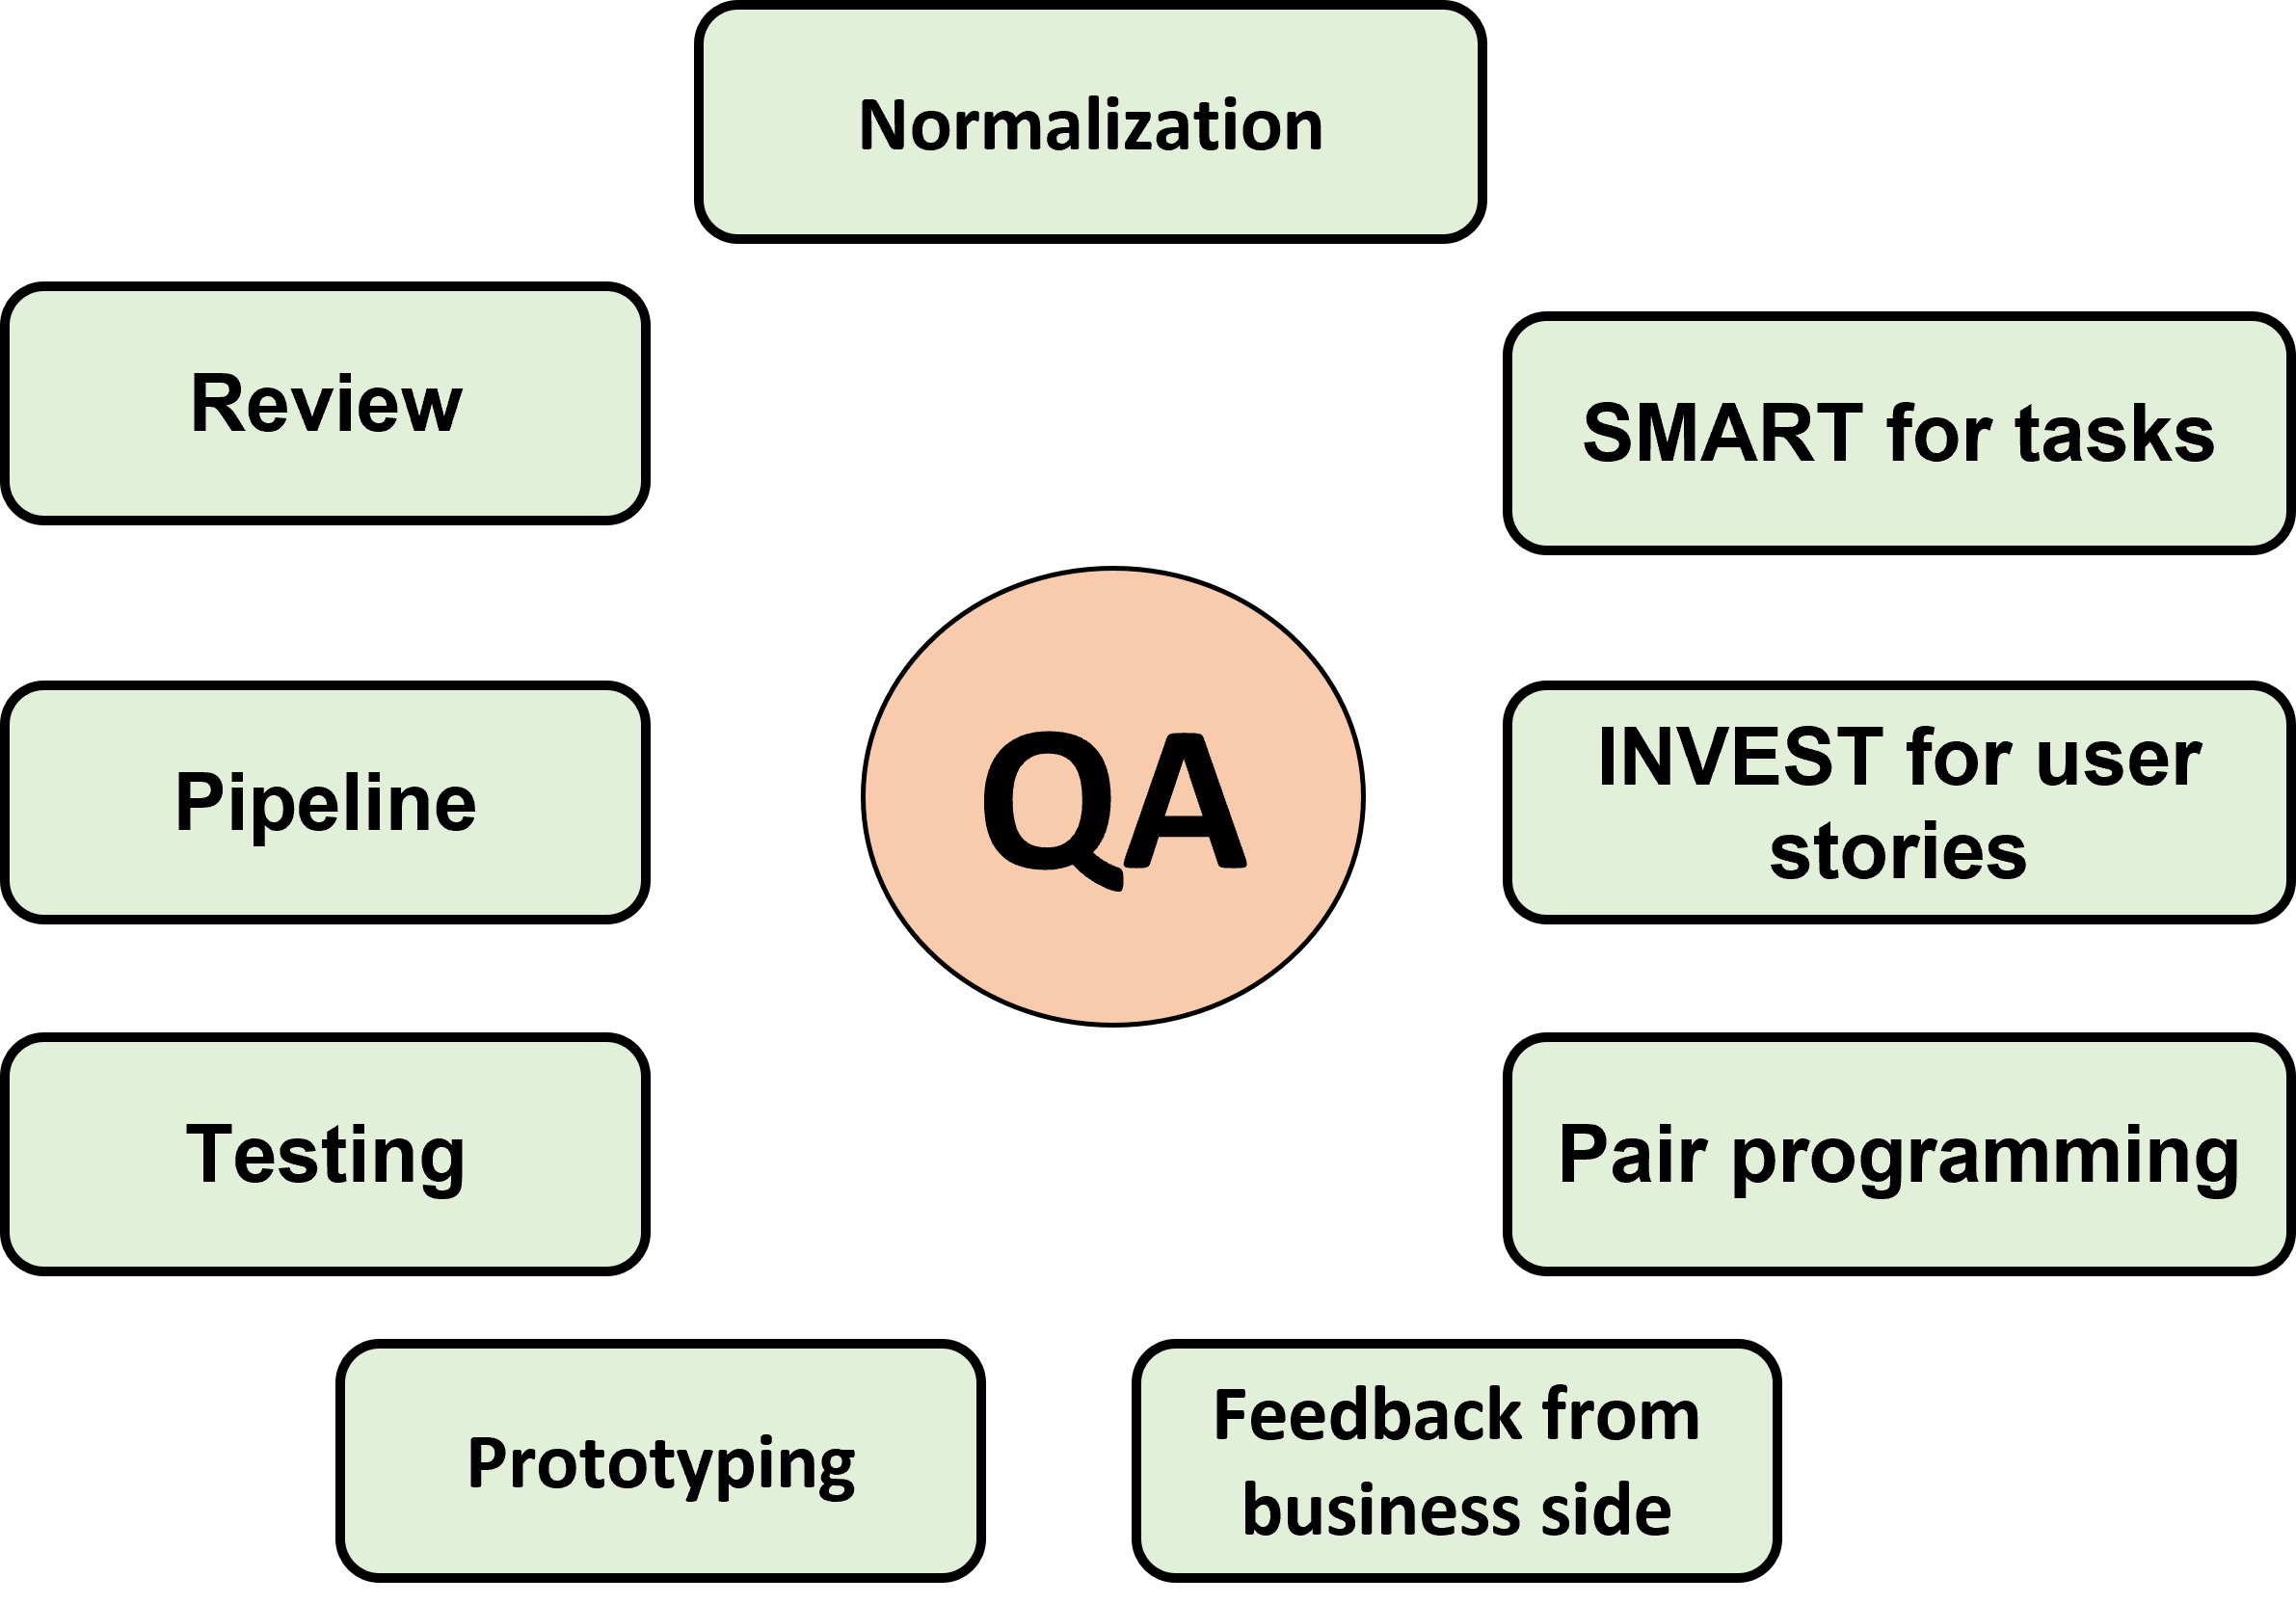
\includegraphics[scale=0.75]{resources/images/qa-techniques.png}
    \caption{QA techniques}
    \label{fig:qa-techniques}
\end{figure}

% % %
\cleardoublepage
\section{Project Review}
\label{sec:project review}

\paragraph{Primary textual contributors.}
\mbox{}\\\emph{Dehom Melissa Pereira Gnassingbe}

\subsection{Development Process}
\emph{How well did your team's development process work, and why? Did the process change between sprints?  In addition, compare and contrast the SCRUM process as practised by your team to (i)~`the' textbook SCRUM process~\cite{scrumbook} and (ii)~the other software development processes presented in module SWT-FSE-B.  Could your team's development process be improved, and by which means?}

\subsection{Team Work}
\emph{How well did your team work together?
Was the distribution of work and the communication among team members effective?
Was the communication with the client effective?}

One of the most positive aspects of our project work was the communication within our group.
From the beginning on, we

\subsection{Lessons Learned}
\emph{What would you change if you could re-start the project, regarding the employed techniques,
    the conduct of the project and any other matters that you consider relevant?  What should stay the same?}

If we could re-start the project, we would give more importance to the traceability of requirements and information in general.
We always made detailed meeting notes and therefore didn't lose information per se.
But on the other hand, it was sometimes hard to remember in which meeting notes to find what we were looking for.
It might have been helpful to extract the information right away, document it in the right place and therefore continuously update our artefacts.
Overall, our documentation represents a point that we could have improved in some places.
Often we were very focused on implementing the features and the focus on documenting was lost.
One example is updating our snowcards.
However, our constant verbal communication allowed us to avoid major issues due to lack of documentation.
Nevertheless, we notice the lack especially now when writing the report.
Also, for formulating and keeping our sprint goal, we would re-take our documentations more often for cross-checking.
Basically, we would take the quality assurance techniques more seriously from the very beginning, since we now understand that there are techniques like object lifecycle diagrams, prototypes and more that can be applied before even implementing some code.
That is one of the biggest lessons learned: Quality assurance doesn't only contain unit and integration tests.
What should stay the same if we re-started the project, is our team spirit and our communication.
In summary, we can say: It was an exciting and challenging project that made us realize to what extent software engineering is a socio-technical discipline.
No matter how well everyone can code: Without teamwork, communication and good project management, the result will not be optimal.





% % %
\cleardoublepage



% Main body of the report (end)
% % % % % % % % % % % % % % % % % % % % % % % % % % % % % % % % %
\cleardoublepage
\fancyhead[RE,LO]{}
\phantomsection
\addcontentsline{toc}{section}{References}
\bibliography{SWL-2021-Report-SWTCamper}


% % % % % % % % % % % % % % % % % % % % % % % % % % % % % % % % %
% Report appendix
\cleardoublepage
\pagestyle{report}

\appendix

\section{Product Backlog}
This section provides information about the user stories that have been completed in each sprint, as well as those not completed and others.

\subsection{Stories Completed in Sprint 1}
\emph{There was no finished story in this sprint.}

\subsection{Stories Completed in Sprint 2}
\emph{Include stories that were completed in the second sprint.}

\subsection{Stories Completed in Sprint 3}
\subsubsection{Login}

\textbf{As a} User,\hfill\break
\textbf{I want} login by supplying my email and my password,\hfill\break
\textbf{so that} I can rent/offer vans or administrate portal.

\textbf{Meta-Information:}
\begin{itemize}
    \item Size: L
    \item Sprint: 3
\end{itemize}

\textbf{Acceptance Criteria:}

The story is done, when
\begin{itemize}
    \item it is impossible to use functionality of portal (other than just looking through offers) without being logged in
    \item wrong username and/or password does not give access (user is informed if password or username is wrong)
    \item a user can change their password in case they've forgotten it and login with the new password
    \item a Renter only sees the renter GUI
    \item a Provider only sees the Provider GUI
    \item a Operator only sees the Operator GUI
    \item it is impossible to use provider functionalities logged in as a provider if the operator has not admitted the registration yet
\end{itemize}

\subsubsection{Registration}

\textbf{As a} User,\hfill\break
\textbf{I want} register by supplying my email and by creation my personal password plus username,\hfill\break
\textbf{so that} I can create a profile at the portal for rent/offer van activities.

\textbf{Meta-Information}
\begin{itemize}
    \item Size: L
    \item Sprint: 3
\end{itemize}

\textbf{Acceptance Criteria}

The story is done, when
\begin{itemize}
    \item only unique emails and usernames are accepted,
    \item only valid usernames and emails are accepted,
    \item only passwords with at least 5 symbols are accepted; otherwise “Password is too short” is displayed
    \item only usernames with at least 5 symbols are accepted; otherwise “Username is too short” is displayed
    \item after successful registration it is possible for the user to login in the portal
    \item after successful registration the user is saved in the database
\end{itemize}


\subsubsection{Request}

\textbf{As a} Renter,\hfill\break
\textbf{I want} to be able to make a request,\hfill\break
\textbf{so that} I know if the wanted vehicle is available.

\textbf{Meta-Information:}
\begin{itemize}
    \item Size: M
    \item Sprint: 3
\end{itemize}

\textbf{Acceptance Criteria:}

The story is done, when
\begin{itemize}
    \item Renter can send a request for booking
    \item New booking is added to the list of all bookings of the renter
\end{itemize}

\subsubsection{Booking}

\textbf{As a} Renter,\hfill\break
\textbf{I want}to be able to make a booking,\hfill\break
\textbf{so that}I can get the wanted vehicle

\textbf{Meta-Information:}
\begin{itemize}
    \item Size: S
    \item Sprint: 3
\end{itemize}

\textbf{Acceptance Criteria:}

The story is done, when
\begin{itemize}
    \item I get a booking confirmation
\end{itemize}

\subsection{Stories Completed in Sprint 4}
\emph{Include stories that were completed in the fourth sprint.}

\subsection{Stories Completed in Sprint 5}
\subsubsection{FAQ}

\textbf{As a} User,\hfill\break
\textbf{I want} to read the FAQ,\hfill\break
\textbf{so that} I can follow the rules of the portal.

\textbf{Meta-Information:}
\begin{itemize}
    \item Size: S
    \item Sprint: 5
\end{itemize}

\textbf{Acceptance Criteria:}

The story is done, when
\begin{itemize}
    \item user can access the FAQ section from the main menu
    \item FAQ consists of all necessary info regarding rent/offer
    \item FAQ section shall be available for all types of users, even for those who are logged out
\end{itemize}


\subsection{Not Completed Stories}
\emph{Include stories that were not completed by the end of the project.}

\subsection{Other Stories}
\emph{Include here stories that were split or combined and do not appear above.}

% % %
\cleardoublepage 



\section{Additional Material}
\begin{figure}[h]
	\centering
	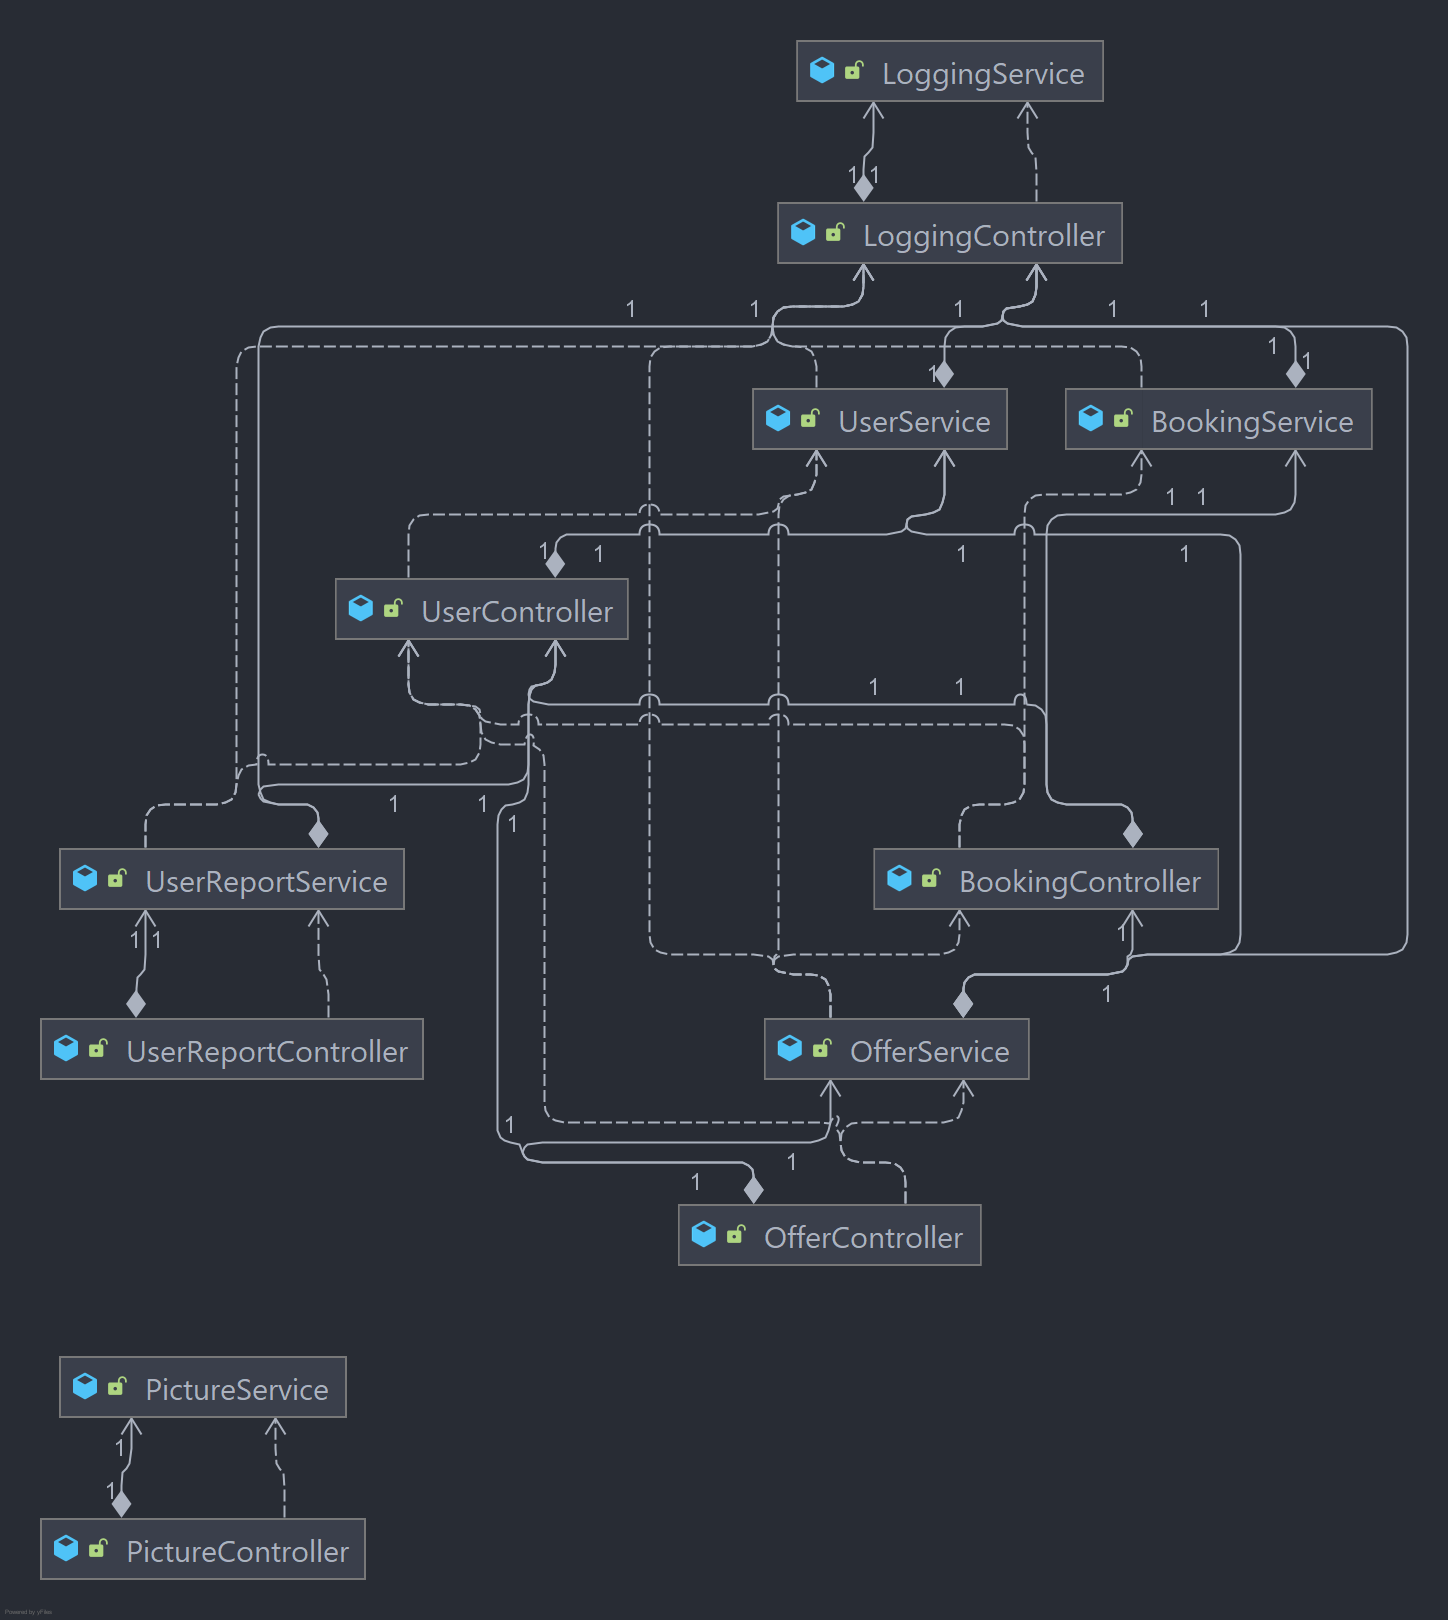
\includegraphics[width=10cm]{resources/images/class diagrams/class-diagram_controller-services.png}
	\caption{Class diagram of Controllers and Services}
	\label{fig:cd:controller-services}
\end{figure}

\begin{figure}[h]
	\centering
	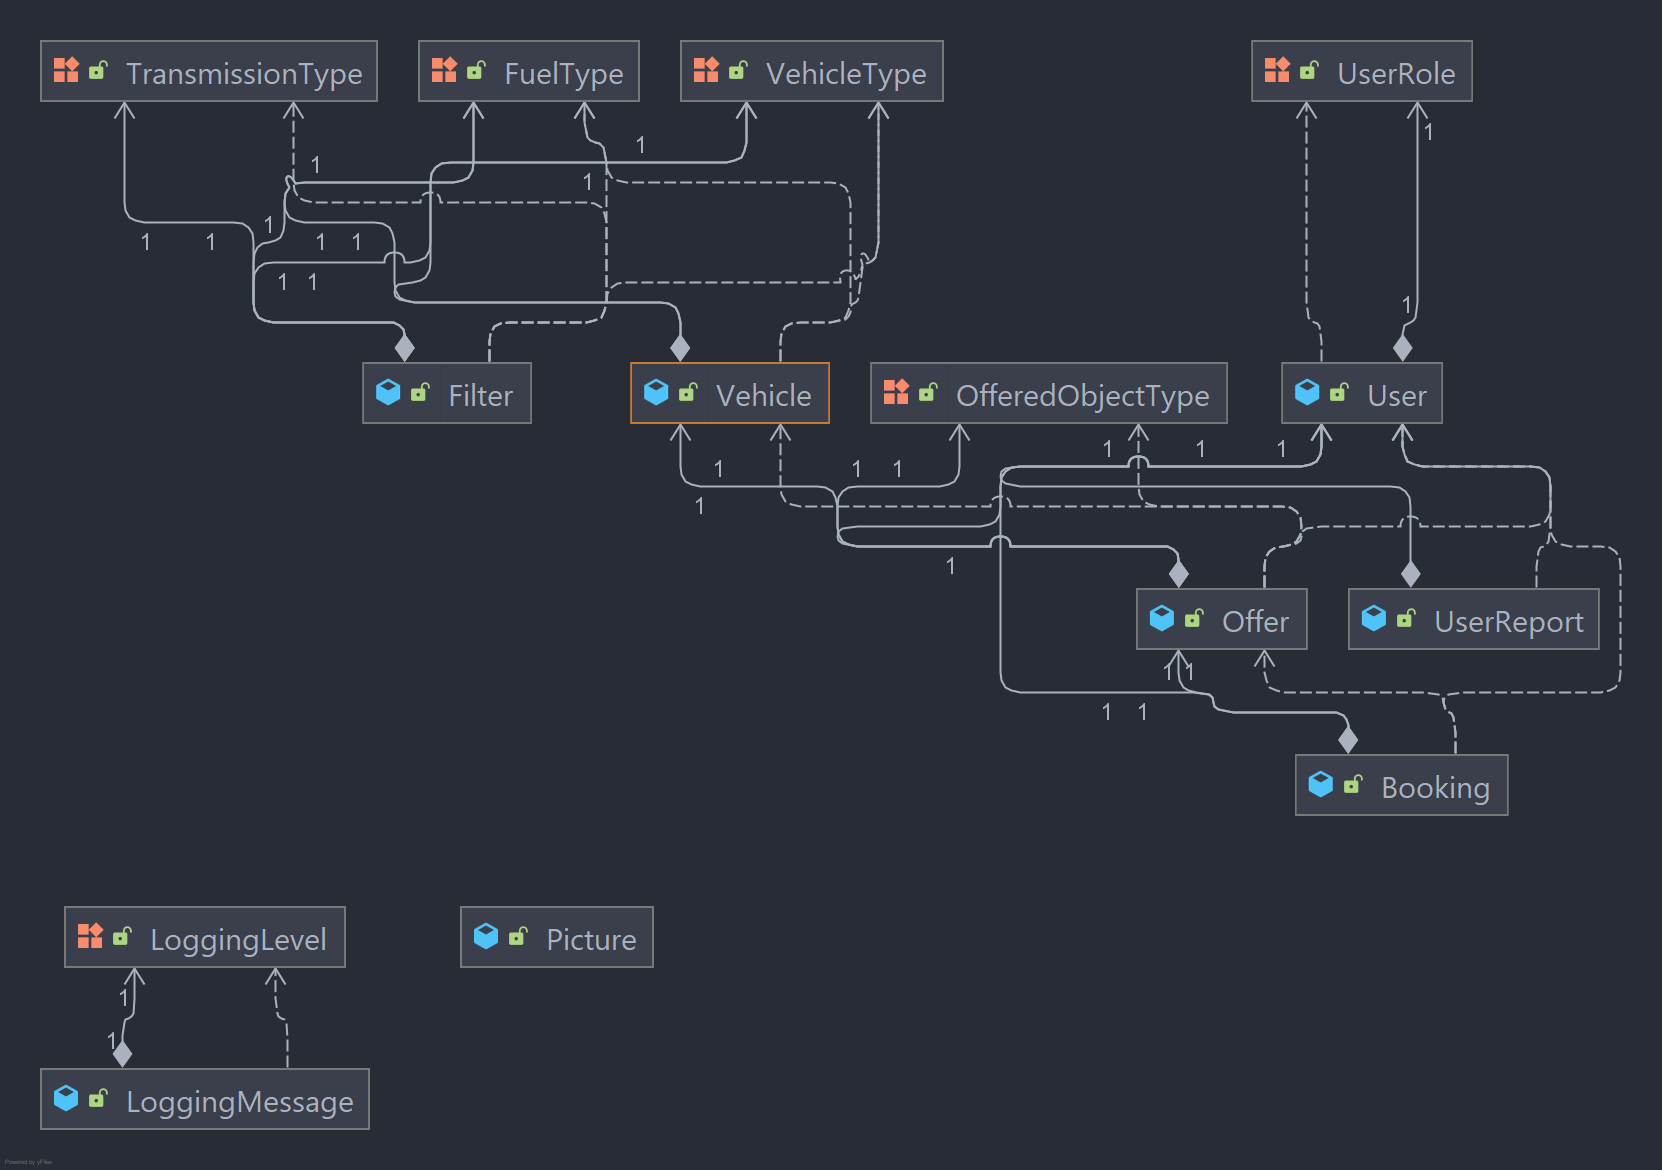
\includegraphics[width=10cm]{resources/images/class diagrams/class-diagram_entities.png}
	\caption{Class diagram of Entities}
	\label{fig:cd:entities}
\end{figure}

\begin{figure}[h]
	\centering
	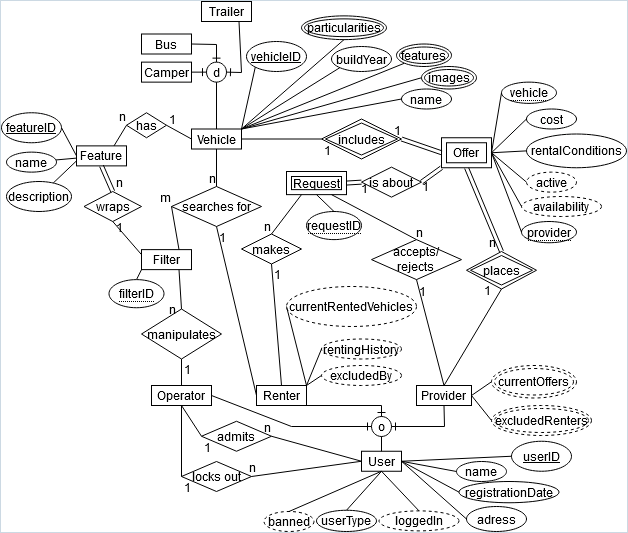
\includegraphics[width=12cm]{resources/images/ER-diagram_first.png}
	\caption{First draft of an Entity Relationship Diagram}
	\label{fig:er-diagram_draft}
\end{figure}

\begin{figure}[h]
	\centering
	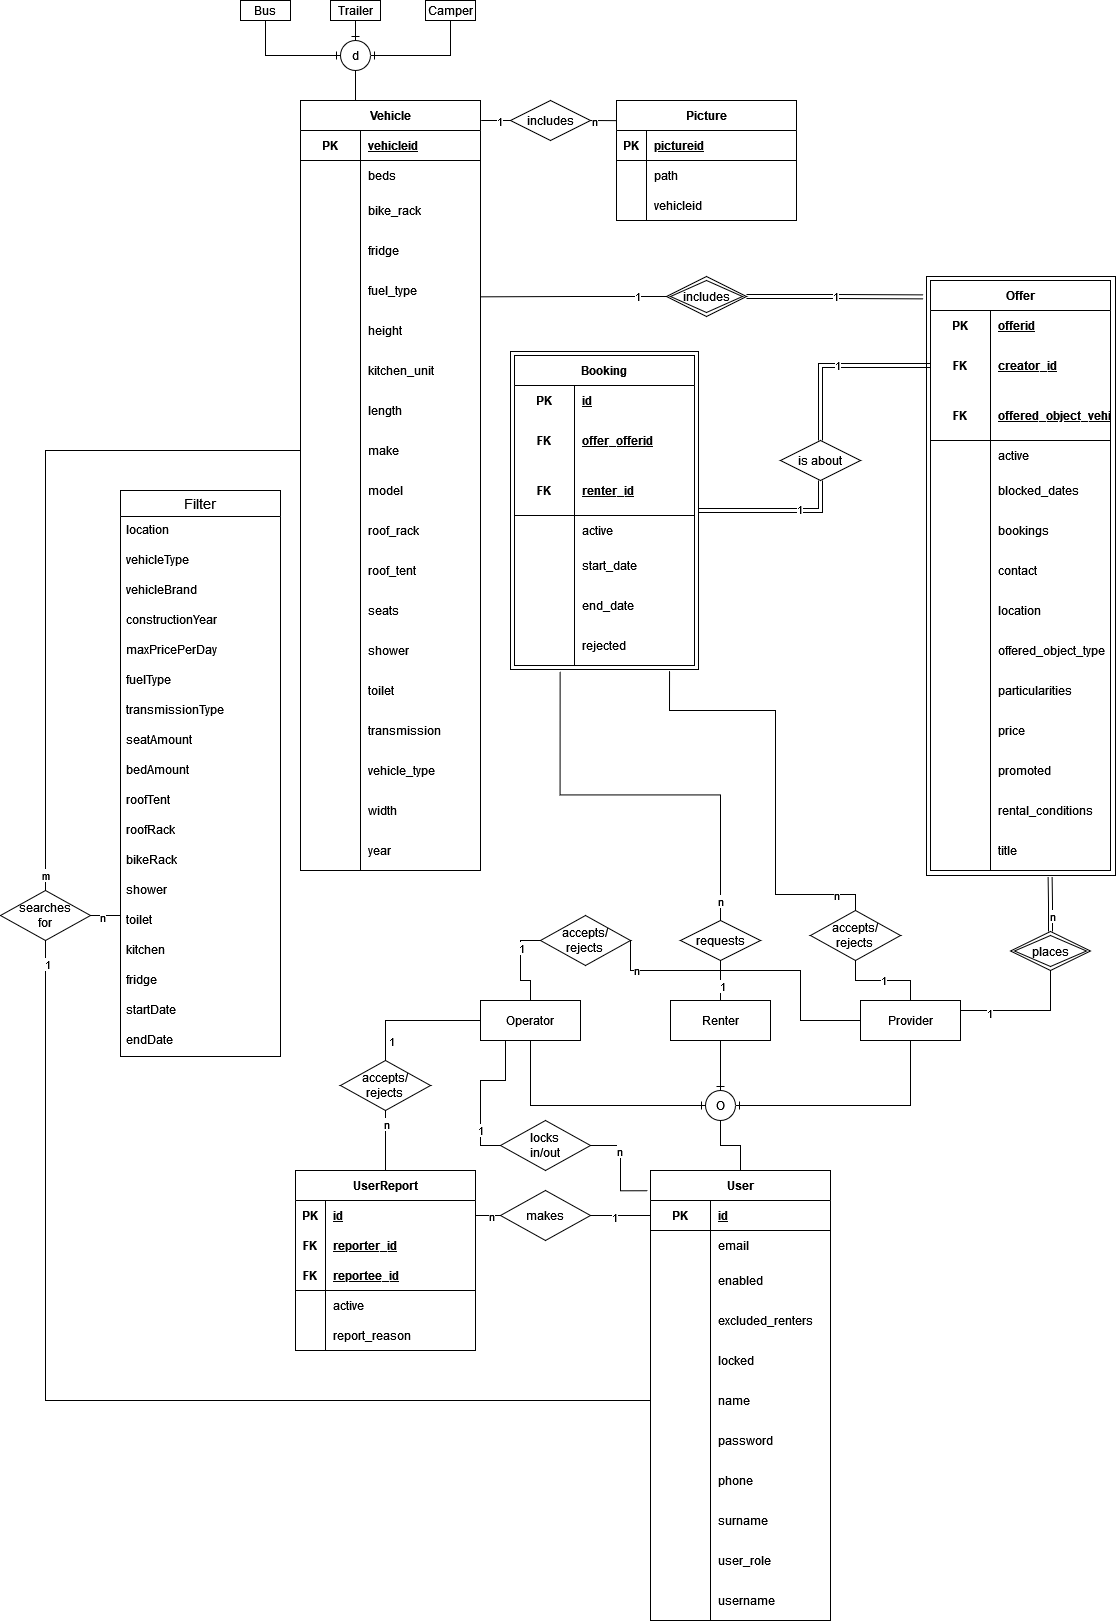
\includegraphics[width=15cm]{resources/images/ER-diagram_final.png}
	\caption{Our final Entity Relationship Diagram}
	\label{fig:er-diagram}
\end{figure}

\begin{figure}[h]
	\centering
	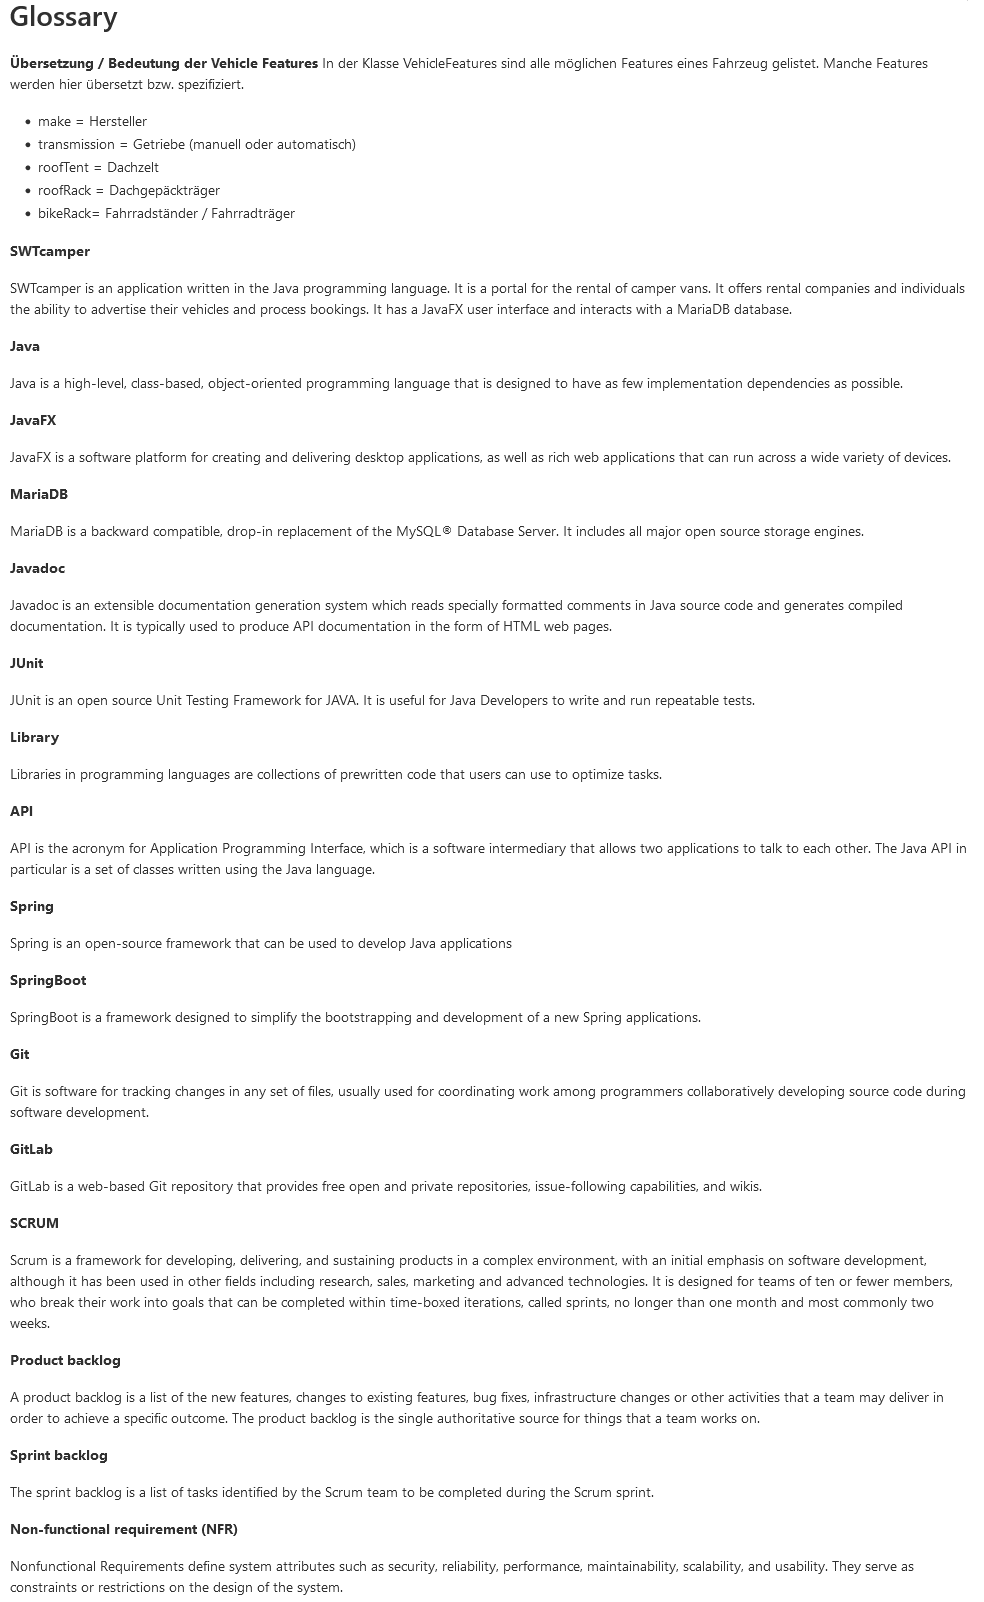
\includegraphics[width=15cm]{resources/images/glossary_1.png}
	\caption{Glossary Part 1}
	\label{fig:glossary_1}
\end{figure}

\begin{figure}[h]
	\centering
	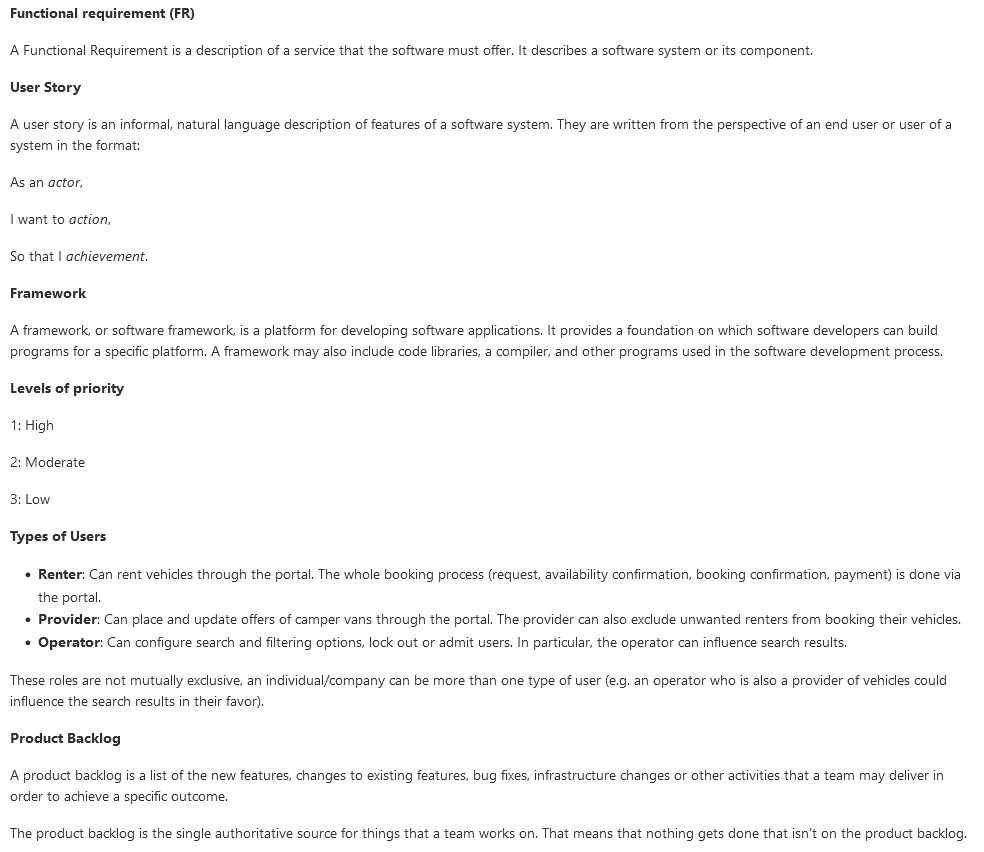
\includegraphics[width=15cm]{resources/images/glossary_2.png}
	\caption{Glossary Part 2}
	\label{fig:glossary_2}
\end{figure}

\begin{figure}[h]
	\centering
	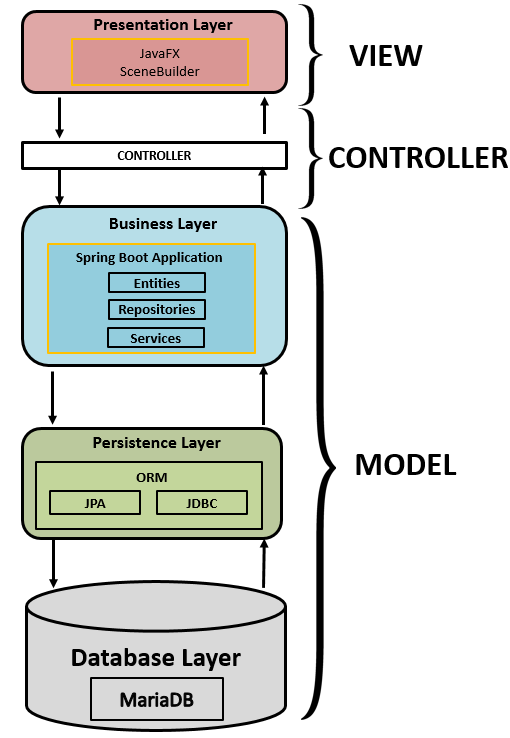
\includegraphics[width=15cm]{resources/images/architecture_early_draft.png}
	\caption{Architecture Diagram (amended after client feedback)}
	\label{fig:architecture_early_draft}
\end{figure}

\begin{figure}[h]
	\centering
	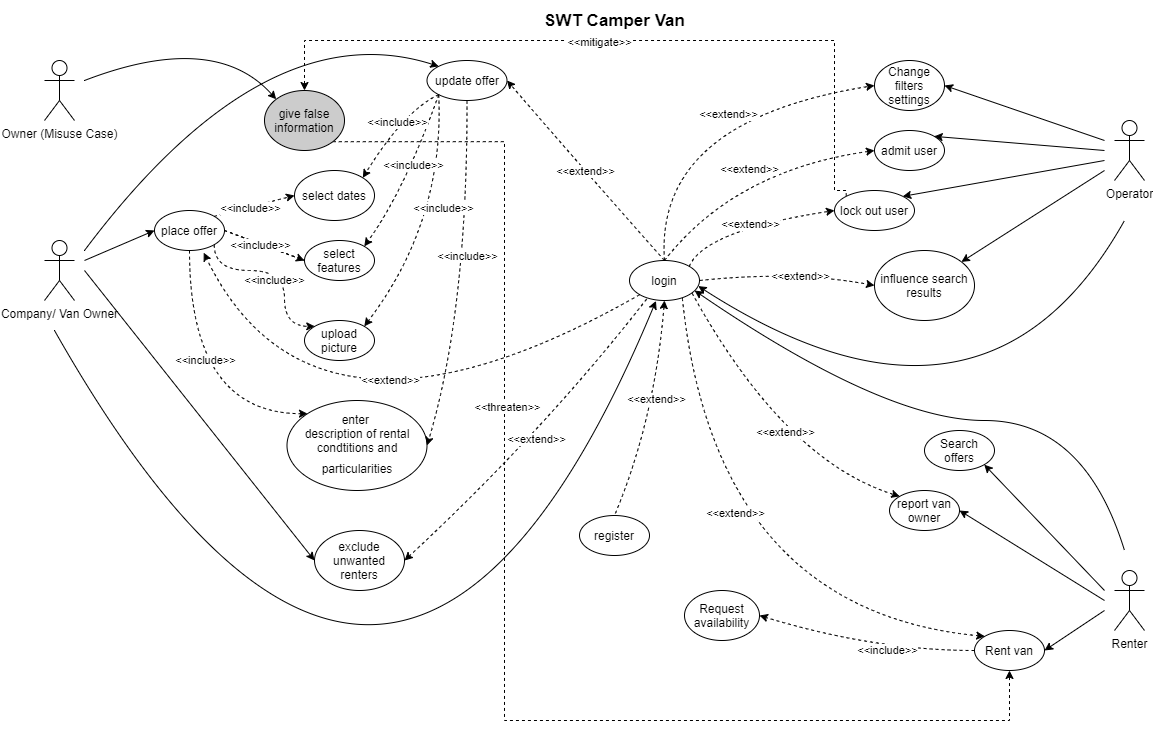
\includegraphics[width=15cm]{resources/images/use-case-diagram.png}
	\caption{Use Case Diagram}
	\label{fig:use-case-diagram}
\end{figure}

\begin{figure}[h]
	\centering
	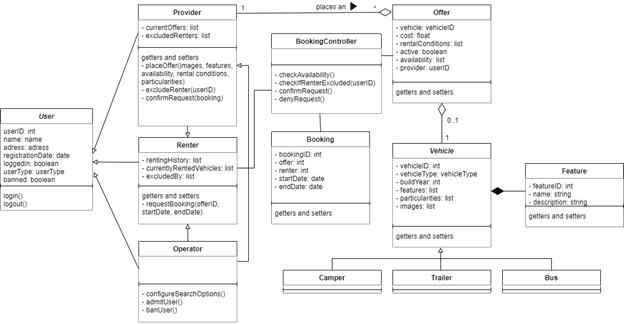
\includegraphics[width=15cm]{resources/images/class_diagram_old.png}
	\caption{Class diagram (discarded after client feedback)}
	\label{fig:class_diagram_old}
\end{figure}

\begin{figure}[h]
	\centering
	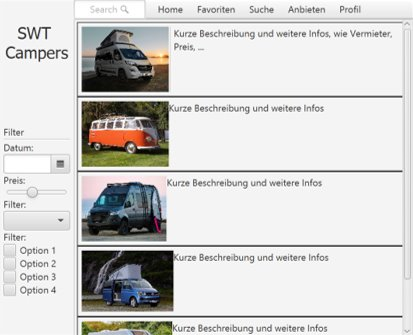
\includegraphics[width=15cm]{resources/images/gui_sketch.png}
	\caption{Early draft of the GUI}
	\label{fig:gui_sketch}
\end{figure}

\begin{figure}[h]
	\centering
	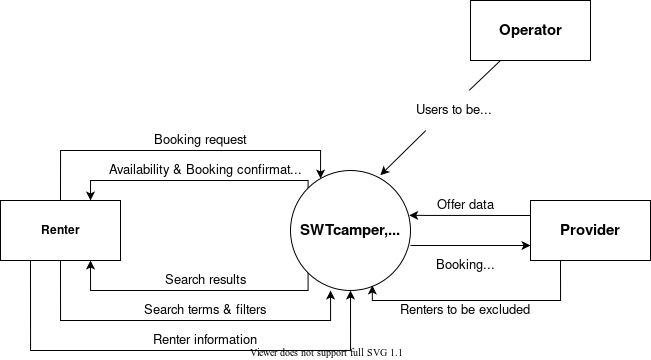
\includegraphics[width=12cm]{resources/images/context_work_diagram.png}
	\caption{Context Work Diagram}
	\label{fig:context_work_diagram}
\end{figure}

\begin{figure}[h]
	\centering
	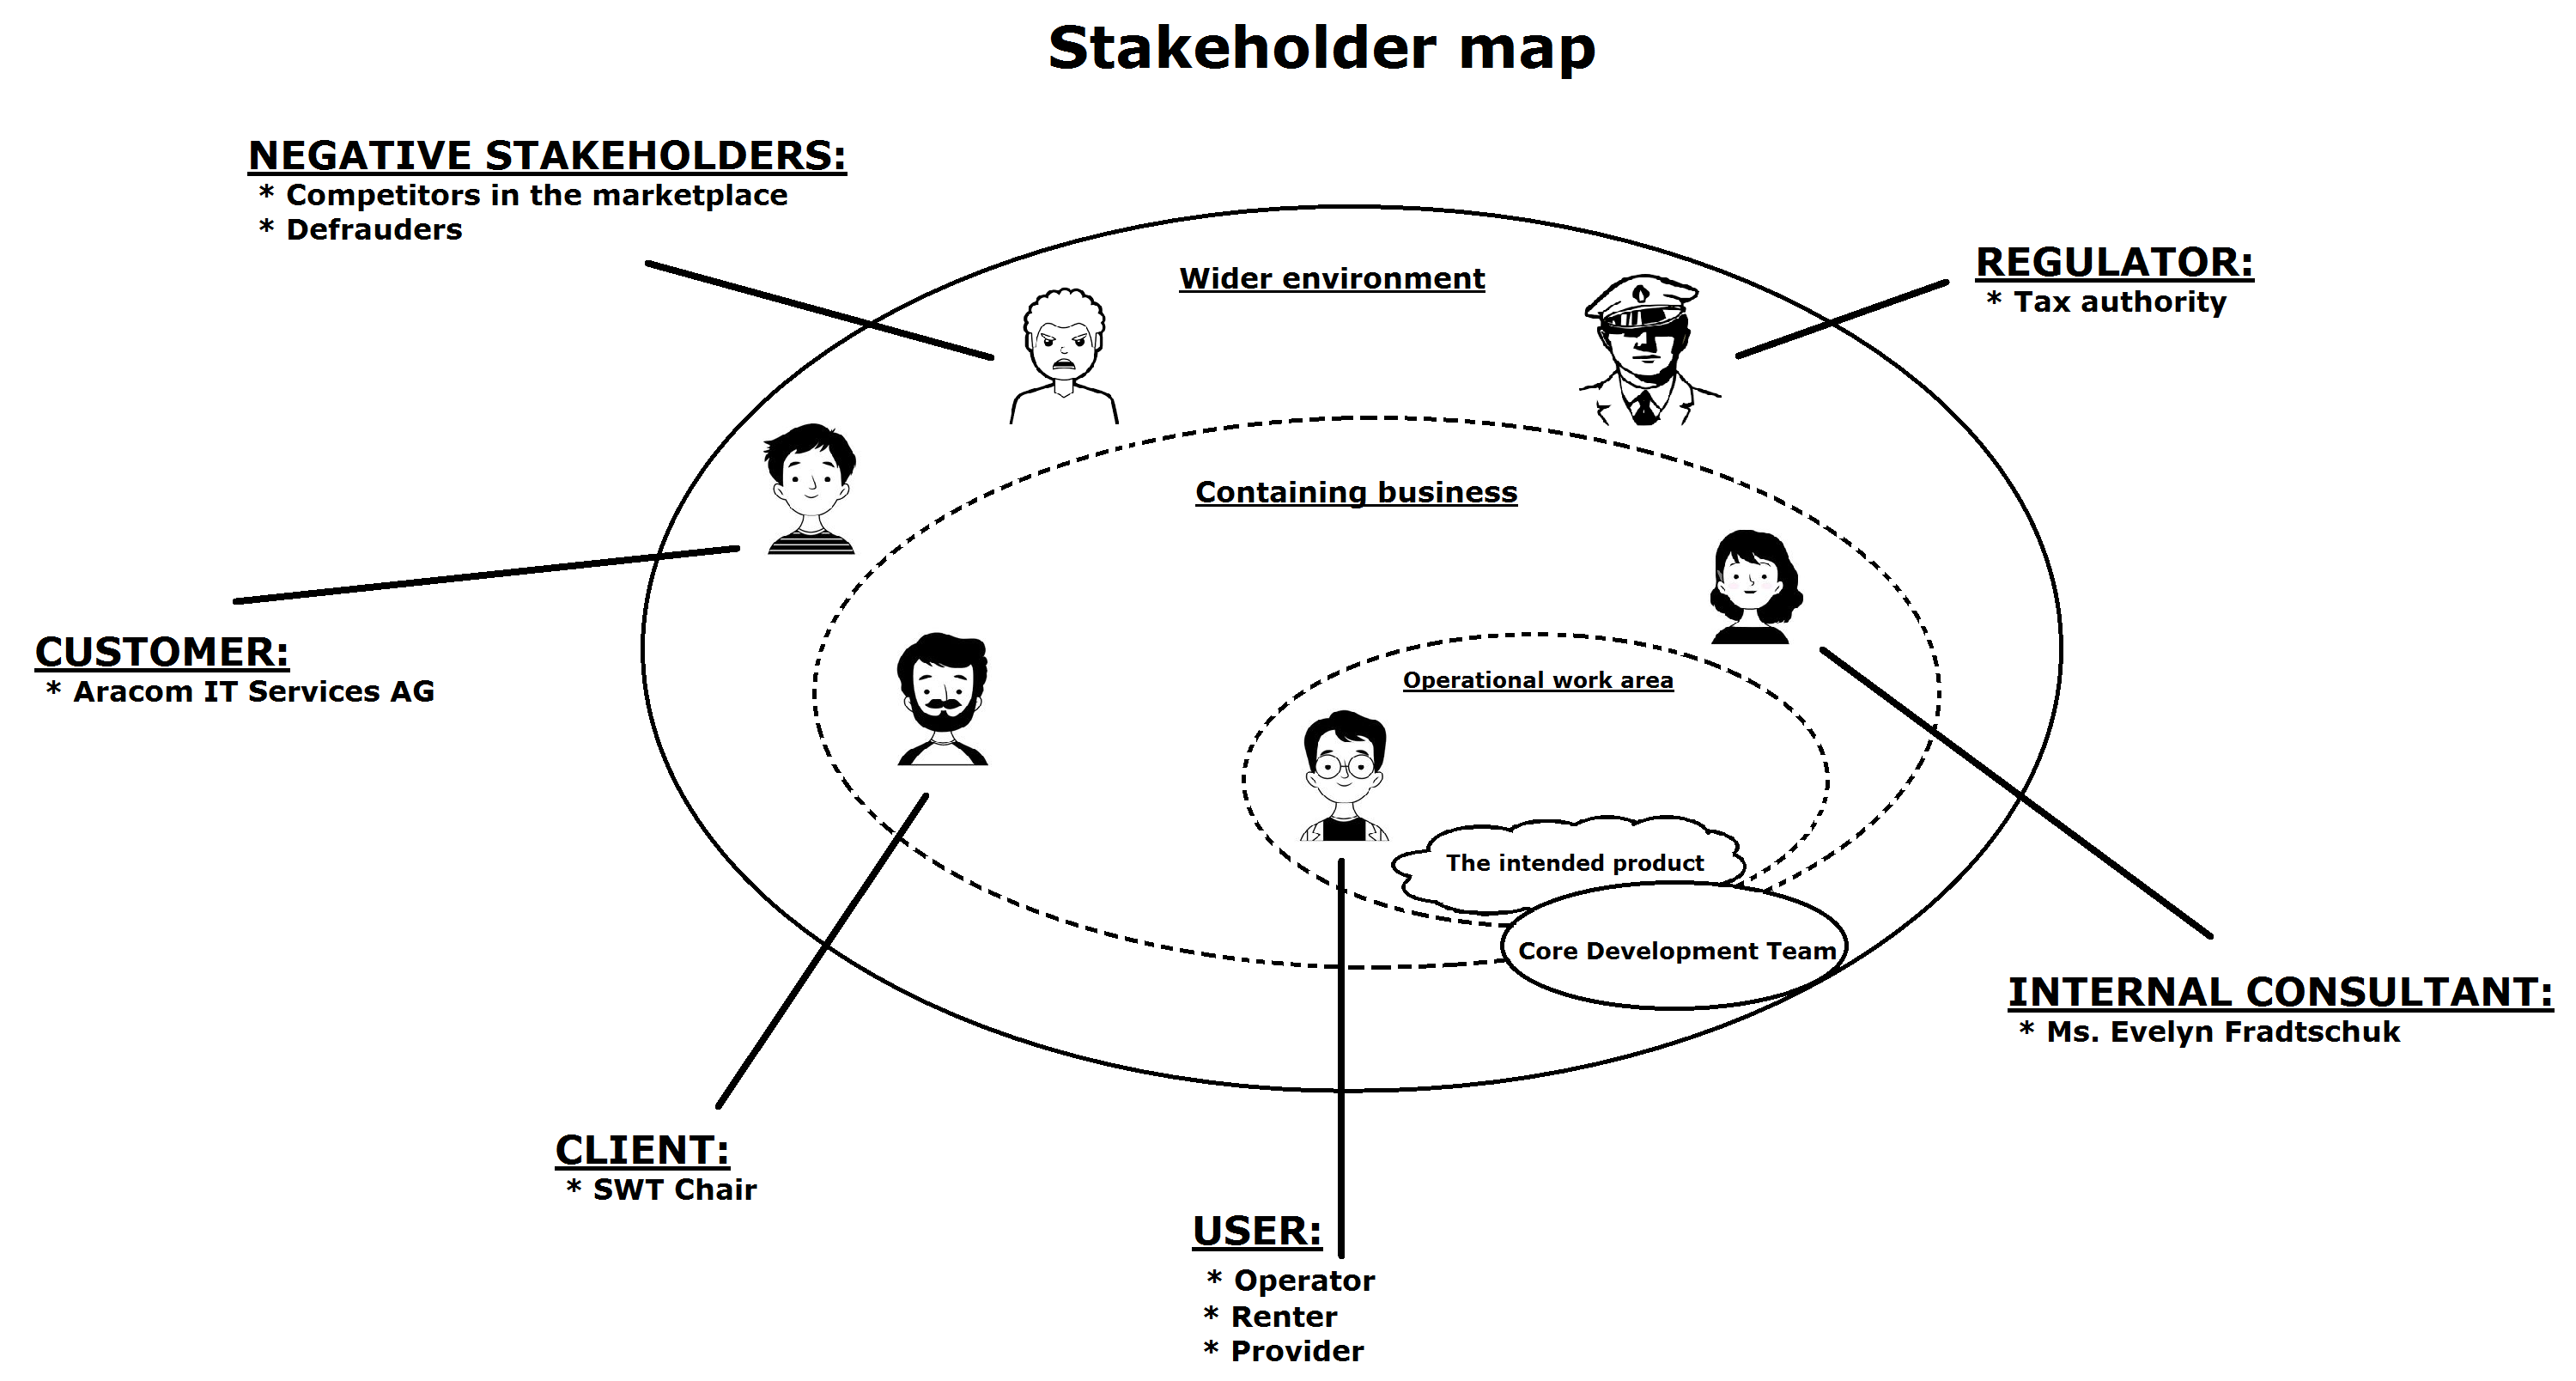
\includegraphics[width=12cm]{resources/images/stakeholder_map.png}
	\caption{Stakeholder Map}
	\label{fig:stakeholder_map}
\end{figure}

\begin{figure}[h]
	\centering
	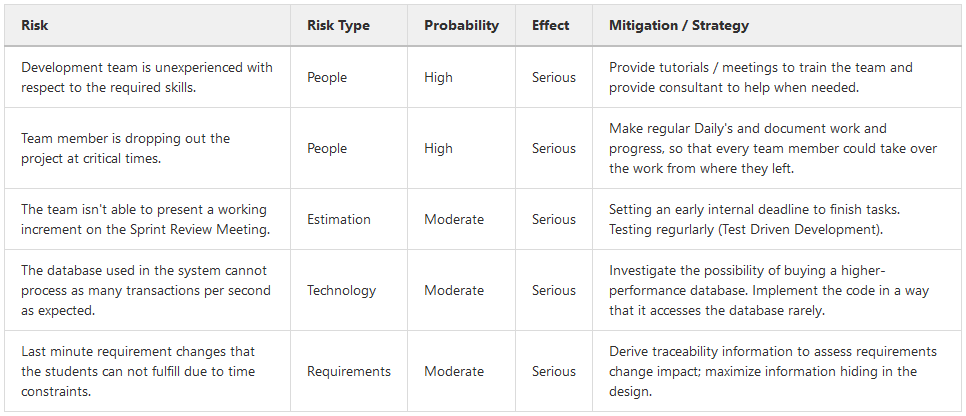
\includegraphics[width=15cm]{resources/images/risks.png}
	\caption{Risks}
	\label{fig:risks}
\end{figure}



% % %
\cleardoublepage


% % % % % % % % % % % % % % % % % % % % % % % % % % % % % % % % %
% Ehrenwörtliche Erklärung (declaration of proper academic conduct)
\cleardoublepage
\phantomsection
\addcontentsline{toc}{section}{Ehrenw\"{o}rtliche Erkl\"{a}rung}
\rhead{Ehrenwörtliche Erklärung}

\section*{Ehrenwörtliche Erklärung}
\label{sec:erklaerung}
Alle Unterzeichner erklären hiermit, dass sie die vorliegende Arbeit
(bestehend aus dem Projektbericht sowie den separat abgelieferten
digitalen Werkbestandteilen) selbständig verfasst und keine anderen als
die angegebenen Quellen und Hilfsmittel benutzt haben.

\studentsignature{Full name of Student 1}

\studentsignature{Full name of Student 2}

\studentsignature{Full name of Student 3}

\studentsignature{Full name of Student 4}

\newpage

\studentsignature{Full name of Student 5}

\studentsignature{Full name of Student 6}

\end{document}
